\documentclass[12pt,a4paper]{report}

\usepackage[utf8]{inputenc}
\usepackage[T1]{fontenc}
\usepackage[francais]{babel}

\usepackage{amsmath,amsthm}
\usepackage{a4wide}

\usepackage{amssymb}

% permet  verbatim de conserverles tabulations
\usepackage{moreverb}

% pour faire des shemas
\usepackage{tikz}
\usepackage{arydshln}
\usepackage{graphicx}

% pour inserer des images
\usepackage{arydshln}


\newtheorem*{rem}{Remarque}
\newtheorem*{ex}{Exemple}
\newtheorem*{q}{Question}
\newtheorem*{schema}{Répresentation}
\newtheorem*{rap}{Rappel}
\newtheorem*{id}{Idée}

\begin{document}

\title{Système d'exploitation\\}
\author{Cours : Raymond Namyst \\ TD : A. Guermouche\\\\ Ecrit par : Marie-Luce ALLEE\\}
\maketitle

\begin{abstract}

\textbf{\textit{Objectif :}} \\
\begin{itemize}
\item "Comment fonctionne un système d'exploitation?"
\item "Pourquoi ça marche comme ça?"
\end{itemize}

\vspace*{2cm}

\textbf{\textit{Notation :} }\\
\begin{description}
\item TP : NACHOS $\rightarrow$ 3 projets à rendre
\item Contrôle continu = ($\frac{Nachos 1 + Nachos 2+ Nachos 3 + DS}{4}$)
\item Note final = MAX ($\frac{CC + EX}{2}$, EX)
\end{description}

\vspace*{2 cm}

\textbf{\textit{Biblio :} }\\
\begin{description}
\item "Système d'Exploitation"  \_ A. Tanenbaum
\item "Structure des système d'exploitation" \_ A.Silberschatz
\item "Le noyau Linux" \_ Bovet \& Cesati
\end{description}

\end{abstract}

\tableofcontents
\newpage

\section*{Contexte}
A l'origine ce qu'on appelait un \textit{système d'exploitation} consistait en un ensemble de routine résidant en mémoire.\\
(Aujourd'hui, on appelle ça une bibliothèque)\\
$\rightarrow$ pilotes de périphériques\\

\textit{\underline{Historiques de l'ordinateur :}}

 
(1945 $\sim$ 55) - Un ordinateur est une salle entière\\
\hspace*{2,8 cm} - \textit{interface} : des interrupteurs puis des cartes\\
\hspace*{2,9 cm}perforées ($\sim$ 50)\\
\hspace*{2,8 cm} - \textit{sortie} : au début des ampoules\\

(1955 $\sim$ 65) - arrivée des transistors\\
\hspace*{2,8 cm} - arrivée des bandes magnétiques\\
\hspace*{2,8 cm} ($\hookrightarrow$ permet de lire aléatoirement les données)\\
\hspace*{2,8 cm} $\rightarrow$ 1$^e$ fois où on parle de "système" \\
\hspace*{1cm} Le "système" est une moniteur qui enchaine les travaux séquentielle-ment.\\

(1965 $\sim$..) - arrivé de la multiprogrammation (plusieurs travaux appartenant à des utilisateurs différents, en même temps en mémoire)\\
\textit{Objectif} : recouvrir les temps d'entrées-sorties\\

\textit{Exemple} de système multitâche : MULTICS (conçu par MIT, Bill, Général Electrics)\\
\hspace*{2cm} 1969 : UNIX




% CHAPITRE 1
\chapter{Introduction aux systèmes d'exploitation}
Un \textit{système}, c'est une machine abstraite qui ajoute des services par rapport à un matériel.
\begin{itemize}
\item arbitrage de l'accès aux ressources
\item virtualisation du matériel
\item primitives de plus haut niveau que le matériel (fichiers, processus, espaces d'adressage,...)
\end{itemize}

\bigskip

\begin{q}
Que se passe t-il au démarrage d'une machine?
\end{q}
\smallskip
\begin{enumerate}
\item Le processeur exécute un programme contenue dans le "BIOS" (Basic Input Output System), code qui se trouve dans une puce mémoire non volatile $\rightarrow$ dans la mémoire morte (ROM) de la carte mère.\\
Le \emph{BIOS} contient le nom du périphérique où se trouve le "système d'exploitation"\\
\begin{rem}
boot : est juste un gestionnaire de système 
\end{rem}
\item Le BIOS charge le "système" en mémoire et l'exécute\\
\hspace*{3,5cm} $\downarrow$\\
\hspace*{3cm} le noyau du système
\end{enumerate}

\medskip

\begin{schema} \end{schema}
\begin{center}
\begin{tikzpicture}
\draw (0,0) circle (0.3) ;
\draw (0,0.2) node[above]{$init$} ;
\draw (1,0) circle (0.3) ;
\draw (1,0.2) node[above]{$shell$} ;
\draw (2,0) circle (0.3) ;
\draw (3,0) circle (0.3) ;
\draw (4,0) node[right]{$\longleftarrow *$} ;
\draw (-1,-0.5) -- (4,-0.5) ;
\draw (1.5,-1) node[below]{$Noyau (code + donnees)$} ;
\draw (4,-1.5) node[right]{$\longleftarrow **$} ;
\draw (-1,-2) -- (4,-2) ;
\draw (1.5,-2) node[below]{$Materiel$} ;
\end{tikzpicture}
\end{center}

\textbf{Légende :\\}
* : processus ($\simeq$ programme binaire en cours d'exécution)\\
** : Dans le Noyau, on y trouve :
\begin{itemize}
\item la gestion de processus
\item la gestion de la mémoire
\item les pilotes de périphériques
\end{itemize}

\begin{rem} : \emph{init} est le premier processus lancé. Il contient l liste des processus à lancer.
\end{rem}

\textbf{{\underline{Démarrage \& gestion des processus}}} \medskip

\begin{tikzpicture}
\draw[->] (0,0) -- (8,0);
\draw (8,0) node[right] {$x$};
\draw[->] (0,0) -- (0,6) ;
\draw (0,1) node[left] {$Bios$};
\draw (0,2) node [left] {$noyau$};
\draw (0,3) node[left] {$init$};
\draw (0,4) node[left] {$P1$};
\draw (0,5) node[left] {$P2$};
\draw (0,6) node[above] {$y$};

\draw (0,1) -- (1,1);
\draw (1,2) -- (2,2);
\draw (2,3) -- (3,3);
\draw (3,2) -- (4,2);
\draw (4,4) -- (5,4);
\draw (5,2) -- (6,2);
\draw (6,5) -- (7,5);
\draw (7,2) -- (8,2);

\draw [dashed] (1,1) -- (1,2);
\draw [dashed] (2,2) -- (2,3);
\draw [dashed] (3,3) -- (3,2);
\draw [dashed] (4,2) -- (4,4);
\draw [dashed] (5,4) -- (5,2);
\draw [dashed] (6,2) -- (6,5);
\draw [dashed] (7,5) -- (7,2);

\draw (0.65,0.90) -- (0.65,1.10);
\draw (0.85,0.90) node[below] {$\uparrow$};
\draw (2.2,0.85) node[below] {\small{$chargement$}};
\draw (2.2,0.55) node[below] {\small{$du$ $noyau$}};
\draw (1.65,1.9) -- (1.65,2.10);
\draw (1.85,1.9) node[above] {$\downarrow$};
\draw (1,2.3) node[above] {\small{$chargement$}};
\draw (1.2,2) node[above] {\small{$d'init$}};

\draw (1,5) node[above] {$mode$};
\draw (1,5) node[below] {$utisateur$};
\draw (3,0) node[below] {$\uparrow $};
\draw (5,0) node[below] {$\uparrow$};
\draw (4,-1) node[above] {$interruption$ $d'horloge$};
\draw (3.5,2) node[below] {$\uparrow$};
\draw (4,1.6) node[below] {$traitement$ $d'horloge$};

\end{tikzpicture}
\medskip
\begin{itemize}
\item Le traitement d'horloge est de très petite durée. 
\item Le noyau lors du traitement d'horloge choisit de redonner la main à init ou à un processus en mode utilisateur (ici P1 ou P2)
\end{itemize}

\medskip

\begin{q}Que fait un processeur lorsqu'il reçoit une interruption?\end{q}
\begin{enumerate}
\item les interruptions sont numérotées
\item l'interruption provoque une sauvegarde des registres et effectue un saut à une adresse qu'il récupère dans la table des vecteurs d'interruption
\end{enumerate}

\medskip
\begin{q}Que ne doit pas pouvoir faire un processus?\end{q}
\begin{itemize}
\item il ne faut pas qu'ils puissent accéder à toute la mémoire
\item il ne faut pas qu'ils aient accès à la totalité du jeu d'instruction du processus\\
\end{itemize}

\bigskip

Les processus fonctionnent selon (au moins) 2 modes :
\begin{itemize}
\item le mode noyau ("privilégié")
\item le mode utilisateur ("protégé")\\
concernant le mode utilisateur, certaines instructions ne sont pas exécutables.
\end{itemize}
Il existe un bit dans un registre du processeur qui permet de configurer le mode\\

Lorsque le processeur tente d'exécuter une instruction illégale, une interruption est déclenchée (SIG ILL)\\
De plus, lors d'une interruption, le processeur passe en mode noyau.\\
Une interruption particulière est réservée aux processus pour lui permettre de basculer volontairement dans le noyau.\\
On appelle ça un appel système ($\simeq$ 300 sur les OS contemporains)\\

Pour indiquer l'appel demandé, le processus utilise un registre.
\medskip
\begin{verbatimtab}
open()
{
 movl 5, %eax
 int 80h      --> passe en mode noyau
}
unistdh
\end{verbatimtab}



% NACHOS
\chapter{NACHOS}
\section{NACHOS est un processus}

\textit{Représentation du processus NACHOS}
\begin{center}
\begin{tikzpicture}
\draw (0,0) ellipse (2 and 3);
\draw (1,2.25) node[right] {$\curvearrowleft$ $processus$};
\draw (-1,1.75) ellipse (0.25 and 0.5);
\draw (0,1.75) ellipse (0.25 and 0.5);
\draw (1,1.75) ellipse (0.25 and 0.5);
\draw (-2,1) -- (2,1);
\draw (1.5,0.5) node[right] {$\longleftarrow$ $interpreteur$ $MIPS$};
\draw (-2,0) -- (2,0);
\draw (1.5,-1) node[right] {$\longleftarrow$ $simulation$ $systeme$ $d'exploittation$};
\draw (-2,-2) -- (2,-2);
\draw (0.75,-2.5) node[right] {$\longleftarrow$ $simulation$ $materiel$ $(memoire,$ $processus,...)$};
\draw [dashed] (-3,-4) -- (3,-4);
\draw (0,-4) node[below] {$noyau$ $linux$};
\draw (-5,-2) rectangle (-4,-1);
\draw (-5, -1.5) node[right] {$halt$};
\draw [>=stealth,->] (-4,-1) -- (-1,1.75);
\end{tikzpicture}
\end{center}

\begin{rem}:\\
\begin{itemize}
\item L'interpréteur MIPS est la pour éviter de passer la main au noyau linux.
\item halt est du binaire
\item NACHOS est un processus récursif
\\
\end{itemize}
\end{rem}

\section{Répertoires principaux dans NACHOS}
\begin{description}
\item nachos/machine/ : processus pour le matériel
\item nachos/thread/ : processus pour le noyau
\item nachos/userprog/ : processus pour la mémoire
\item nachos/text/
\\
\end{description}
\bigskip

\textbf{Description des répertoires plus en détail :\\}

$\bullet$ Répertoire thread
\begin{verbatimtab}
cd nachos/thread
./nachos
\end{verbatimtab}
Résultat de ces commandes : le noyau est lancé puis un test se fait pour vérifier si le noyau marche puis le processus s’éteint

\bigskip
$\bullet$ Répertoire userprog
\begin{verbatimtab}
cd nachos/userprog
./nachos -x ../test/halt/   --> lance le programme halt sur Nachos

 main()
{
 Halt();
}
\end{verbatimtab}

Que fait Halt()?? \\
Son code se trouve dans nachos/test/start.s (.s : c'est de l'assembleur)\\
\begin{verbatimtab}
Halt : addiu SC$\_$Halt, \$0, \$2     --> en IA-32 : mov SC$\_$Halt, r2
       syscall
       j 31            --> équivaut à un return
\end{verbatimtab}

\begin{rem}Assembleur MIPS a été choisit car c'est l'assembleur le plus simple.\end{rem}

\bigskip

$\bullet$ Dans nachos/test/, on trouve tous les programmes utilisateurs\\
Ces programmes doivent donc être en MIPS, on utilise donc un compilateur "croisé" qui génère du code MIPS\\

$\bullet$ fonction ExceptionHandler()
nachos/userprog/exception.cc a une fonction ExceptionHandler()
\begin{verbatim}
ExceptionHandler()  
{
regarde quel erreur, appel système est appelé
.
.
switch(n)
..
 case SC_Halt() := exit();
 case : <ERREUR>
..
}
\end{verbatim}

$\bullet$ Pour modéliser la mémoire machine, un tableau est utilisé $\rightarrow$ mainMemory[..]


\section{Représentation matériel de NACHOS :} 
\begin{itemize}
\item Machine\\
(registre MIPS + mémoire + ...)
\item Interrupt
\item Console
(Entrée / Sortie)
\\
\end{itemize}

$\bullet$ \textit{Représentation du système dans NACHOS\\}
Nachos possède les classes suivantes:
\begin{itemize}
\item Thread
\item Scheduler\\
Il maintient une liste de processeurs, c'est lui qui choisit qui prend la main après une interruption = ordonnancement
\item Semaphore\\
Sert à la synchronisation
\item AddrSpace\\
$\rightarrow$ représente l'espace mémoire des processus
\end{itemize}


% CHAPTER 3
\chapter{Gestion de processus}

\begin{rap} un processus est une instance de programme en cours
 d'exécution. \end{rap}

\textbf{Représentation de l'espace d'adressage d'un processus :}
\begin{center}
\begin{tikzpicture}
\draw (0,0.5) ellipse (2 and 3.5) ;
\draw (-1,-2) rectangle (1,3) ;
\draw (-1,-1) -- (1,-1) ;
\draw[dashed] (-1,-0.5) -- (1,-0.5) ;
\draw (-1,0) -- (1,0) ;
\draw (-1,1) -- (1,1) ;
\draw (-1,2) -- (1,2) ;

\draw (-0.25,1) node[right] {$\uparrow$} ;
\draw (-1,1.5) node[right] {$?$} ;
\draw (-0.25,2) node[right] {$\downarrow$} ;

\draw (1,-1.5) node[right] {$code$ $=$ $programme$ $(+$ $bibliotheques)$} ;
\draw (1,-0.5) node[right] {$donnees$} ;
\draw (1,0.5) node[right] {$tas$} ;
\draw (1,2.5) node[right] {$pile$} ;
\draw (1.65,2) node[right] {$\longleftarrow$ $espace$ $d'adressage$} ;
\draw (3,1.5) node[right] {$=$ $ensemble$ $des$ $memoires$ $"qu'il$ $voit"$} ;
\draw (3,1) node[right] {$(adresses$ $virtuelles)$};
\end{tikzpicture}
\end{center}

\begin{rap}
\begin{itemize}
\item le code et une partie des données sont chargés en mémoire au démarrage du processus.
\item les bibliothèques sont chargées que lors de leur première utilisation, c'est-à-dire pas forcément toutes au démarrage. (Raison : les bibliothèques sont de très gros fichiers).
\item le tas est un segment de données.
\\
\end{itemize}
\end{rap}

$\bullet$ Zoom sur la partie "?" :\\
Comment est organisé cette partie?

\medskip

\begin{center}
\begin{tikzpicture}
\draw (-0.25,1) -- (2.25,1);
\draw[thick] (0,2) rectangle (2,3);
\draw (-0.25,4) -- (2.25,4);
\draw (-0.25,5) -- (2.25,5);
\draw (-0.25,6) -- (2.25,6);

\draw (0,0.25) -- (0, 4);
\draw (0,5) -- (0, 6.5);
\draw (2,0.25) -- (2, 4);
\draw (2,5) -- (2, 6.5);

\draw (2,0.5) node[right] {$tas$};
\draw (0.5,1) node[right] {$\uparrow$};
\draw (2,2.5) node[right] {$bibliotheques$};
\draw (2,4.5) node[right] {$il$ $y$ $a$ $des$ $trous$ $/memoire$ $discontinue$};
\draw (0.5,6) node[right] {$\downarrow$};
\draw (2,6.5) node[right] {$pile$};
\end{tikzpicture}
\end{center}


$\bullet$ Le noyau alloue une structure pour chaque processus dans laquelle il stocke :
\begin{itemize}
\item un pid : indice ds le tableau pour savoir ou il est
\item une priorité
\item une sauvegarde des registres
\item un couple : utilisateur réel (celui qui a lancé le processus)/ utilisateur effectif
\item une cartographie mémoire du processus (pour savoir une fois le processus fini ce qu'on peut libérer comme mémoire ou encore quelle taille maxime peut être donner à ce processus)
\end{itemize}

\medskip

\begin{schema} \end{schema}
\begin{center}
\begin{tikzpicture}
\draw (0,0) ellipse (1 and 2);
\draw (-0.5, -0.5) rectangle (0.5,1.5);
\draw (-2,-0.75) -- (2,-0.75);
\draw (-.25,-1.85) rectangle (0.25, -0.85);
\draw (-0.25,-.95) -- (0.25, -0.95);
\draw (-0.25,-1.1) -- (0.25, -1.1);
\draw (-0.25,-1.25) -- (0.25, -1.25);
\draw (-0.25,-1.4) -- (0.25, -1.4);

\draw (-1,-1.5) node[left] {$noyau$};
\draw[->] (0.2,-1.75) -- (2,-1.15);
\draw (2,-1) node[right] {$pointeur$ $dans$ $le$ $noyau$ $pour$ $gerer$};
\draw (2,-1.5) node[right] {$des$ $fichiers$ $par$ $exemple$};

\end{tikzpicture}
\end{center}

\newpage

\section{Différents états d'un processus}
\begin{center}
\begin{tikzpicture}
\draw (0,0) circle(1);
\draw (-1.1,0) node[right] {$naissance$};
\draw [->] (1,0) -- (2,0);
\draw (3,0) circle(1);
\draw (2.5,0) node[right] {$pret$};
\draw [->](3.9,0.5) -- (6.6,0.5);
\draw (3.8,1) node[right] {\small{$choisit$ $par$}};
\draw (3.7,0.7) node[right] {\small{$ordonnencement$}} ;
\draw [<-](3.9,-0.5) -- (6.6,-0.5);
\draw (4.2,-0.75) node[right] {\small{$preempte$}};
\draw (7.5,0) circle(1);
\draw (6.9,0) node[right] {$actif$};
\draw [->] (8.5,0) -- (9.5,0);
\draw (10.5,0) circle(1);
\draw (9.9,0) node[right] {$bloque$};
\draw (11.2,-0.5) node[right] {\small{$en$ $attente$}};
\draw (11,-0.85) node[right] {\small{$d'une$ $entree/sortie$}};
\draw[<-] (3,-1) -- (3,-2) -- (10.5,-2) -- (10.5,-1);
\draw (6.5, -2) node[below] {\small{$E/S$ $termine$}};

\draw [dashed] (-2,2) -- (13,2);

\draw (7.5,4) circle(1);
\draw (7,4) node[right] {$actif$};
\draw [->] (7,0.9) -- (7,3.1);
\draw [<-] (8,0.9) -- (8,3.1);
\draw (8,2.75) node[right] {\small{$appel$ $systeme$}};
\draw (8,2.25) node[right] {\small{$ou$ $interruption$}};

\draw (-2.2,2.5) node[right] {$utilisateur$} ;
\draw (-2.2,1.5) node[right] {$noyau$};
\end{tikzpicture}
\end{center}

\begin{rem}
\begin{itemize}
\item Le nombre de processus actifs en même temps $\leq$ au nombre de cœur sur la machine.
\item Même lors d'un appel système, le noyau peut décider de passer la main à un autre processus.
\item Préempté : les registres du processus actif sont enregistrés puis le processus est remis en prêt.
\item Exemple d'un processus bloqué : emacs\\
Comment sort un processus de l'état bloqué?
\begin{enumerate}
\item[$\ast$] processus actif : gcc, processus bloqué : emacs
\item l'utilisateur tape sur une touche $\rightarrow$ interruption
\item gcc passe alors en noyau \& réveille emacs qui passe en processus
\item le noyau fait l'échange entre emacs et gcc
\end{enumerate}
\end{itemize}
\end{rem}

\medskip

La transition entre l'état actif et l'état prêt s'appelle un \emph{changement de contexte} (switch$\_$to)
\begin{verbatim}
switch_to(Thread *current, Thread *next)
{

- sauver les registre du processus dans la structure current
- charge les valeurs de la structure next dans les registres

}
\end{verbatim}

\medskip

En réalité, dans un noyau tout est thread. Les processus n'existent plus (ils ont disparus dans les années 2000)\\
Les threads stockent la même chose qu'un processus, la cryptographie mémoire en moins.\\

Quelques différences :
\begin{itemize}
\item Il existe des threads qui n'agissent que dans le noyau, d'autres entre  le noyau $\&$ dans le mode utilisateur.
\item Deux threads peuvent avoir un même espace d'adressage.
\item La mémoire est représentée dans AddrSpace.\\
\end{itemize}

\begin{schema} \end{schema}
\medskip
\begin{center}
\begin{tikzpicture}
\draw (0,0) rectangle (1,0.5);
\draw (-0.5,-0.25) node[right] {$AddrSpace$};
\draw[<-,thick] (1,0.25) -- (2,0.25);

\draw (2,0) rectangle (3,0.5);
\draw (2,0.25) node[right] {$t_1$};
\draw[->] (3,0.25) -- (3.5,0.25) ;
\draw (3.5,0) rectangle (4.5,0.5);
\draw (3.5,0.25) node[right] {$t_2$};
\draw[->] (4.5,0.25) -- (5,0.25);
\draw (5,0) rectangle (6,0.5);
\draw (5,0.25) node[right] {$t_3$};
\draw[->] (6,0.25) -- (6.5,0.25);
\draw[->] (5.5,0) -- (5.5,-0.5) -- (9,-0.5) -- (9,0);
\draw (6.5,0) rectangle (7.5,0.5);
\draw (6.5,0.25) node[right] {$t_4$};
\draw[->, thick] (7.5,0.25) -- (8.5,0.25);

\draw (8.5,0) rectangle (9.5,0.5);
\draw (9,-0.25) node[right] {$AddrSpace$};

\draw[dashed] (-1,1) -- (11,1);
\draw (-1,1) node[below] {$noyau$};

\draw (2,2) ellipse (0.5 and 0.7);
\draw (2,2.7) node[above] {$\downarrow$};
\draw (2.5,3) node[above] {$espace$ $d'adressage$};
\draw (6,2) ellipse (0.5 and 0.7);

\draw[thick] (2,1.3) -- (2.5,.5);
\draw[thick] (1.8,1.4) -- (.5,.5);
\draw[thick] (6,1.3) -- (5.5,.5);
\draw[thick] (6,1.3) -- (7,.5);
\draw[thick] (6.5,1.8) -- (9,.5);
\end{tikzpicture}
\end{center}

\section{Ordonnancement des processus}
L'ordonnancement des processus est un compromis entre :
\begin{itemize}
\item maximiser l'occupation du processus
\item le système doit être le plus interactif possible
\item les calculs doivent être les plus performants possibles (ex : compilation rapide)
\end{itemize}

\medskip

\subsection{Ordonnancement le plus simple à mettre en œuvre : FIFO (First In, First Out}
\medskip
\begin{center}
\begin{tikzpicture}
\draw (2,0.25) node[left] {$liste$ $des$ $threads$ $pret$ $\longrightarrow$} ;
\draw (2,0) rectangle (3,0.5);
\draw[->] (3,0.25) -- (3.5,0.25) ;
\draw (3.5,0) rectangle (4.5,0.5);
\draw[->] (4.5,0.25) -- (5,0.25) ;
\draw (5,0) rectangle (6,0.5);
\draw[dashed,->] (6,0.25) -- (6.5,0.25) ;
\draw[dashed] (6.5,0) rectangle (7.5,0.5);

\end{tikzpicture}
\end{center}
\medskip

Lorsque le processus actif meurt ou se bloque, il est retiré de la liste et on passe au nouveau premier de la liste.\\
Les nouveaux processus sont rajoutés à la fin de la liste.\\
On trouve ce genre d'ordonnancement dans NACHOS (justement!) ou encore dans les JVM (Java Virtual Machine)\\

\textbf{Point négatif : } risque de famine.\\
Le premier processus peut faire une boucle sans fin par exemple.

\subsection{FIFO + horloge qui provoque des changements de contexte = tourniquet (Round Robin)}

\begin{schema} \end{schema}
\begin{center}
\begin{tikzpicture}
\draw (0,0) rectangle (0.5,0.5);
\draw[->] (0,0.25) -- (-0.75,1);
\draw (-1,1) rectangle (-0.5, 1.5);
\draw[->] (-0.75,1.5) -- (-0.75,2);
\draw (-1,2) rectangle (-0.5, 2.5);
\draw[->] (-.75,2.5) -- (0,3.25);
\draw (0,3) rectangle (0.5, 3.5);
\draw[->] (0.5,3.25) -- (1.25,2.5);
\draw (1,2) rectangle (1.5,2.5);
\draw[->] (1.25,2) -- (1.25,1.5);
\draw (1,1) rectangle (1.5, 1.5);
\draw[->] (1.25,1) -- (0.5,0.25);
\end{tikzpicture}
\end{center}

\begin{q}Est-ce que UNIX pourrait être comme ça? \end{q}
Imaginons qu'il y ait 100 processus. Un des processus est Firefox (dont l'action est la lecture d'une vidéo), si on lui donne la main qu'après les 100 autres processus : il n'aura la main que 10ms toutes les secondes. Ce n'est bien évidement pas possible.\\

\begin{description}
\item \textbf{Point positif :} plus de famine
\item \textbf{Point négatif :} pas d'interactivité
\end{description}

\subsection{Algorithme avec file de priorité}

\begin{center}
\begin{tikzpicture}
\draw (0,0) rectangle (2,4);
\draw (0,0.5) -- (2,0.5);
\draw (0,1) -- (2,1);
\draw (0,1.5) -- (2,1.5);
\draw (0,2) -- (2,2);
\draw (0,2.5) -- (2,2.5);
\draw (0,3) -- (2,3);
\draw (0,3.5) -- (2,3.5);

\draw[->] (1.5, 0.25) -- (3,0.25);
\draw (3,0) rectangle (3.5,0.5);
\draw[->] (3.5, 0.25) -- (4, 0.25);
\draw (4,0) rectangle (4.5,0.5);
\draw (4.5,0.5) node[right] {$ex$ $:$ $gcc,$ $demon$ $d'impression...$ $\longleftarrow$ $tache$ $de$ $fond$} ;

\draw[->] (1.5, 2.75) -- (3,2.75);
\draw (3,2.5) rectangle (3.5,3);
\draw[->] (3.5, 2.75) -- (4, 2.75);
\draw (4,2.5) rectangle (4.5,3);
\draw[->] (4.5, 2.75) -- (5, 2.75);
\draw (5,2.5) rectangle (5.5,3);
\draw (5.5,3) node[right] {$ex$ $:$ $firefox$} ;

\draw[->] (1.5, 3.75) -- (3,3.75);
\draw (3,3.5) rectangle (3.5,4);
\draw[->] (3.5, 3.75) -- (4, 3.75);
\draw (4,3.5) rectangle (4.5,4);
\draw (4.5,4) node[right] {$ex$ $:$ $emacs,$ $shell$} ;

\draw (0,0) node[left] {$priorite$ $Min$} ;
\draw (0,4) node[left] {$priorite$ $Max$} ;

\end{tikzpicture}
\end{center}
Chaque processus a une priorité fixe.\\

$\Rightarrow$ utilisé pour les systèmes à temps-réel (ex: dispositif de pilotage)\\

Pour UNIX : \\
Il est difficile d'ordonnancer les processus. On ne sait pas le faire.\\
\begin{ex}Firefox est embêtant, on ne sait pas ce qu'il va faire : google, vidéo (ce qui donne des priorités différentes).\end{ex}

\begin{id} Pour faire un système interactif, il faudrait pouvoir "modifier dynamiquement" les priorités.\end{id}

\subsection{Algorithme utilisés au sein des systèmes de "traitement par lots" (batch)}
\textbf{Objectif :} Minimiser le temps de restitution moyen\\
$\rightarrow$ temps de restitution moyen = temps$\_$de$\_$fin - temps$\_$de$\_$soumission\\

Supposons qu'on ait quatre taches : a,b,c,d\\
durée de taches : t$_a$, t$_b$, t$_c$, t$_d$\\
Si le système exécute a puis b, puis c, et enfin d, alors : \\
\hspace*{1cm} temps restitution(a) = t$_a$\\
\hspace*{1cm} temps restitution(b) = t$_a$ + t$_b$\\
\hspace*{1cm} temps restitution(c) = t$_a$ + t$_b$ +t$_c$\\
\hspace*{1cm} temps restitution(d) = t$_a$ + t$_b$ +t$_c$ + t$_d$\\
\hspace*{2cm} moyen = $\frac{4t_a + 3t_b + 2t_c + t_d}{4}$\\
\hspace*{2.5cm} $\hookrightarrow$ c'est minimal ssi t$_a$ $<$ t$_b$ $<$ t$_c$ $<$ t$_d$\\

\begin{id}estimer la durée du prochain cycle d'utilisateur du CPU en s'appuyant sur le passé (une moyenne du passé)\end{id}

Estimation$_n$ = $\alpha$ . durée$\_$observée$_{n-1}$ + (1-$\alpha$) Estimation$_{n-1}$\\

$\alpha$ = $\frac{1}{2}$,  E= $\frac{1}{2}$ . durée$_{n-1}$ + $\frac{1}{4}$  . durée$_{n-2}$ + $\frac{1}{8}$ . durée$_{n-3}$ + ...

\begin{center}
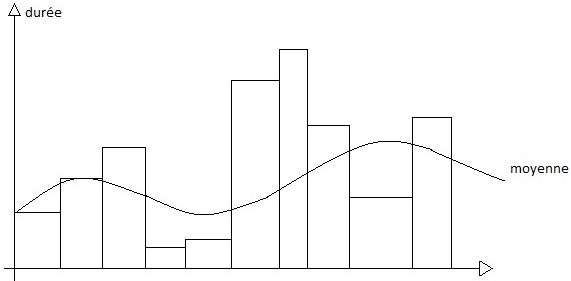
\includegraphics[scale=.7]{./images/schema2_2_4_1.jpg}
\end{center}
\begin{id} La priorité est inversement proportionnelle à l'estimation (on favorise les plus courts) {\large /! $\setminus$} lorsque le processus n'est pas actif, il faut continuer à atténuer son estimation.\end{id}

\begin{ex} Linux 2.4\end{ex}

Sous UNIX, la priorité d'un processus comporte deux aspects :
\begin{enumerate}
\item priorité statique (nice)
\item priorité dynamique : dépend du comportement du processus
\end{enumerate}


Sous Linux,la priorité statique donne droit à un certain nombre de quanta de temps durant une époque.\\

Données initiales : \\
P$_1$ : 5 crédits \textbf{$\rightarrow 4 \rightarrow 3 \rightarrow 2 \rightarrow 1 \rightarrow \emptyset$} \hspace*{1cm} $\mid$ 5\\
P$_2$ : 4 crédits \textbf{$\rightarrow 3 \rightarrow 2 \rightarrow 1 \rightarrow \emptyset$} \hspace*{1.88cm} $\mid$ 4\\
P$_3$ : 2 crédits \textbf{$\rightarrow 1 \rightarrow \emptyset$} \hspace*{3.6cm} $\mid$ 2
\begin{center}
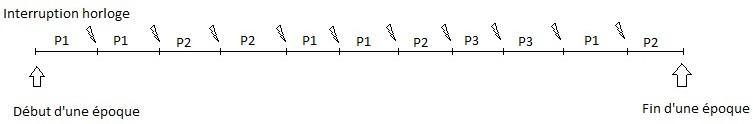
\includegraphics[scale=.6]{./images/schema2_2_4_2.jpg}
\end{center}

\begin{enumerate}
\item P$_1$ : 5$\rightarrow$ 4 : P$_1$ a droit à une deuxième tranche de temps.
\item P$_1$ : 4 $\rightarrow$ 3 \& P$_2$ : 3 :Égalité des priorités entre P$_1$ et P$_2$. P$_1$ est choisit car certaines données sont déjà dans la mémoire cache.
\item ...\\
\end{enumerate}

\textit{Cas où P2 se bloque :}\\

Données initiales : \\
P$_1$ : 5 crédits \textbf{$\rightarrow 4 \rightarrow 3 ... \rightarrow \emptyset$} \hspace*{1.05cm} $\mid$ 5\\
(P$_2$) : 4 crédits \hspace*{3.68cm} $\mid$ 4 + $\frac{4}{2}$\\
P$_3$ : 2 crédits \textbf{$... \rightarrow \emptyset$} \hspace*{2.65cm} $\mid$ 2
\begin{center}
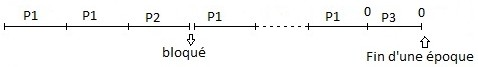
\includegraphics[scale=.8]{./images/schema2_2_4_3.jpg}
\end{center}


A la fin d'une époque, on donne à chaque processus :\\
$$\frac{credit restant}{2} + credits initiaux $$

 $$\Rightarrow \frac{c +\frac{c + \frac{C}{2}}{2}}{2} + C \rightarrow c + \frac{C}{2} +  \frac{C}{4} + ... \l 2C$$

\subsection{Système utilisé dans UNIX (av)}
\textbf{Problème} : lorsque le nombre de processeurs augmente, l'algorithme devient cher. Chaque processeur exécute un goodness sur chaque prêt. On a donc un ensemble de données partagées qui doivent être accéder "un par un".\\
Si il y a plusieurs (milliers) de processeurs, ils ne peuvent pas scheduler en même temps.\\

$\Rightarrow$ il faut synchroniser\\

\textbf{Solution :} on casse la liste de processus en petits morceaux qu'on donne à chaque processeurs.\\
D'autres problèmes sont tout de même à gérer.\\

Il faut partager équitablement $\rightarrow$ la priorité moyenne doit être la même sur tous les processeurs\\
Il se peut aussi que toutes les taches soit finies sur un CPU. Dans ce cas il faut gérer les "voles" de taches aux autres processeurs tout en gardant une vision globale sur les priorités (même si moins précise que lorsqu'il y a un unique processeur).

\section{Synchronisation}
\subsection{Préemption, concurrence, parallélisme}
\begin{description}
\item \textit{Préemption :} le fait d'interrompre un thread/processus et de le retirer du processeur
\item \textit{Concurrence :} l'exécution qui est "entrelacé" de plusieurs threads/processus
\item \textit{Parallélisme :} lorsque plusieurs threads/processus progressent simultanément sur des processus différents\\
\end{description}

Regardons comment NACHOS fonctionne :
\begin{itemize}
\item préemption? \\
./nachos -rs $<$seed$>$ : permet de demander des interruptions d'horloge ($<$seed$>$ pour créer un générateur de nombres aléatoires)\\
$\hookrightarrow$ essaye de créer un currentThread $\rightarrow$ Yield(); ($\rightarrow$ préemption)\\

Dans beaucoup de fonctions de NACHOS :
\medskip
\begin{verbatim}
{ 
  int oldlevel = interrupt -> setLeveel(IntOff);  <- de manière indirecte, 
   .                                               interrupt -> oneTick();
   .
   .
  interrupt ->setLevel(oldLevel);
}
\end{verbatim}
\medskip
Arrêt des interruptions d'horloge dans ce code. \\


\item concurrence : oui
\item parallélisme : non (raison : déterminisme)\\
\end{itemize}

\begin{q} Quel est le principal problème posé par la concurrence entre threads? (c'est-à-dire des processus qui partagent de la mémoire)\end{q}
Lorsque les threads accèdent à une même donnée de manière concurrente (ex : malloc/free, malloc gère une liste de chainées).\\

\begin{ex} manipulation de listes chainées\end{ex}
Insertion de deux threads à peu prés en même temps :
\begin{center}
\begin{tikzpicture}
\draw[blue] (0,1) node[right] {$thread$};
\draw[red] (0,-1) node[right] {$thread$};
\draw[->] (0,0) -- (1,0);
\draw (1,-0.25) rectangle (2,.25);
\draw (1.75,-.25) -- (1.75,.25);
\draw[->] (1.9,0) -- (3,0);
\draw (3,-0.25) rectangle (4,.25);
\draw (3.75,-.25) -- (3.75,.25);

\draw (5,-0.25) rectangle (6,.25);
\draw (5.75,-.25) -- (5.75,.25);
\draw [blue] (3.9,0.75) node[left] {$3$};
\draw[->, blue] (3.85,0) -- (3.85,1) -- (4,1);
\draw [blue] (4.5,1.25) node[above] {$1$};
\draw[blue] (4,1.25) rectangle (5,0.75);
\draw[blue] (4.75,1.25) -- (4.75,.75);
\draw [blue] (4.85,0.5) node[right] {$2$};
\draw[->, blue] (4.85,1) -- (5.25,1) -- (5.25,0.25);

\draw[->] (3.9,0) -- (5,0);
\draw[red] (4.35,.15) -- (4.65, -.15);
\draw[red] (4.35,-.15) -- (4.65, .15);

\draw [red] (3.9,-0.75) node[left] {$3$};
\draw[->, red] (3.85,0) -- (3.85,-1) -- (4,-1);
\draw[blue] (3.7,-.65) -- (4,-.35);
\draw[blue] (3.7,-.35) -- (4,-.65);

\draw [red] (4.5,-1.25) node[below] {$1$};
\draw[red] (4,-1.25) rectangle (5,-0.75);
\draw[red] (4.75,-1.25) -- (4.75,-.75);
\draw [red] (4.85,-0.5) node[right] {$2$};
\draw[->, red] (4.85,-1) -- (5.25,-1) -- (5.25,-0.25);;

\draw[->] (5.9,0) -- (7,0);
\draw (7,-0.25) rectangle (8,.25);
\draw (7.75,-.25) -- (7.75,.25);
\end{tikzpicture}
\end{center}
Résultat : \\

\begin{center}
\begin{tikzpicture}
\draw[->] (0,0) -- (1,0);
\draw (1,-0.25) rectangle (2,.25);
\draw (1.75,-.25) -- (1.75,.25);
\draw[->] (1.9,0) -- (3,0);
\draw (3,-0.25) rectangle (4,.25);
\draw (3.75,-.25) -- (3.75,.25);
\draw[->, blue] (3.9,0) -- (5,0);
\draw[blue] (5,-0.25) rectangle (6,.25);
\draw[blue] (5.75,-.25) -- (5.75,.25);
\draw[red] (5,-1.25) rectangle (6,-0.75);
\draw[red] (5.75,-1.25) -- (5.75,-.75);
\draw[->, red] (5.9,-1) -- (7,0);
\draw[->] (5.9,0) -- (7,0);
\draw (7,-0.25) rectangle (8,.25);
\draw (7.75,-.25) -- (7.75,.25);
\end{tikzpicture}
\end{center}

$\rightarrow$ les modifications de la liste \underline{ne doivent pas} s'effectuer en même temps.\\

\begin{ex} d'une instruction simple exécutée en même temps.\end{ex}
\begin{verbatimtab}
                           int = 0;
thread 1                                thread 2
for (i=0; i$<$100; i++)                 for (i=0; i$<$100; i++)
    n++;                                     n++;

                        peint n? 200 : 100
\end{verbatimtab}
En C : n++, en assembleur $\left\{\begin{array}{l} load @n, r1\\ inc r1 \\ save r1,@n
\end{array} \right.$
Si pas toujours synchrone on pourrait penser que 100$<$ n $<$ 200\\

\begin{center}
\begin{tabular}{lp{4cm}p{4cm}l}
& thread 1 & thread 2 & \\
& lad r & &\\
n=1 & & &\\
\hdashline
& & lad r & ) \\
& & inc r1 & ) x99\\
& & save r1 & )$\rightarrow$ n=99\\
\hdashline
n=1 & save r1 & & \\
\hdashline
& & load r1 & \\
& & inc r1 & \\
\hdashline
99 x ( & & &\\
\hdashline
& & save r1 & n=2\\
\\
& 2 $\leq$ n $\leq$ 200 
\end{tabular}
\end{center}

$\Rightarrow$ même une instruction telle que "n++" doit être exécutée en prenant des précautions!\\
n++ n'est pas une instruction "atomique".\\
Une instruction \emph{atomique} est une instruction qu'un processeur sait exécuter d'un seul tenant, c'est-à-dire qui est non interruptible ni "entrelaçable"\\

Pour résoudre ce problème, on crée une section critique. \\

\subsection{Section critique}
\textit{Section critique :} portion de code qui ne doit être  exécuter que par au plus un thread à la fois.

 \medskip
\begin{verbatim}
bool occupé = FALSE;

entrer_sc()         <------ le premier thread "passe" 
{                            les autres attendent
 while(occupé == TRUE) ;
 occupé =TRUE;
}

sortir_sc()
{
 occupé = FALSE;
}
\end{verbatim}
\medskip
Problème si deux treads/processus passent \verb?occupé? à TRUE en même temps, le problème n'est pas résolu.\\


$\bullet$ Solution (Peterson) pour deux threads
\medskip
\begin{verbatim}
bool drapeau[2] = {FALSE,FALSE};
int tour = 0;

thread i
entrer_sc()
{
  drapeau[i] = TRUE;
  tour = i;
  attendre(drapeau[1-i] == FALSE ou tour == 1-i);  //1-i = "l'autre"
}

sortir_sc()
{
  drapeau[i] = FALSE;
}
\end{verbatim}
\medskip
La variable \verb?tour? joue le rôle de l'arbitre et désigne qui est arrivé en dernier.\\

Généraliser "Peterson" à n processus est possible, mais c'est couteux et limité à un nombre de processus bornés.\\
$\rightarrow$ les architectes ont introduit de nouvelles instructions dans le processus\\

\begin{ex} l'instruction "test and set"\end{ex}
\begin{verbatim}
int test_and_set(int *verrou)
{
 int old = *verrou;
 *verrou = 1;
 return old;
}
\end{verbatim}
\medskip

$\Longrightarrow$ test$\_$and$\_$set : instruction atomique

\medskip
\begin{verbatim}
enter_sc()
{
  while(test_and_set(&verrou) == 1);
}

sortir_sc()
{
 verrou = 0;
}
\end{verbatim}
\medskip

\textbf{Amélioration :}
\smallskip
\begin{verbatim}
entrer_sc()
{
  while(test_and_set(&verrou) == 1)
     while(verrou == 1);
}
\end{verbatim}
\bigskip

Mais il reste encore quelques problèmes.\\
Explication sur un exemple :
\begin{center}
\begin{tabular}{c c c c}
thread 0 & thread 1 & thread 2 & thread 3 \\
$\mid$ & $\mid$ & $\mid$ & $\mid$ \\
$\mid$ SC $\mid$ & $\circlearrowleft$ & $\mid$ & $\mid$\\
$\mid$ & & & \\
$\mid$ CPU $\mid$ & $\mid$ CPU $\mid$ & & \\
\end{tabular}
\end{center}

\begin{itemize}
\item pour le thread 1 : gaspillage d'un quantum de temps à chaque fois qu'il est ordonné.
\item pour le thread 0 : le détendeur d'une section critique peut être préempté \\
\\
\end{itemize}

Test$\_$and$\_$Set : instruction utilisée comme brique de base pour construire des schémas de synchronisation plus complexe
\begin{description}
\item$\ominus$ interférences avec l'ordonnancement
\item$\ominus$ attente active
\item$\ominus$ synchronisation plus complexe\\
\end{description}

\subsection{Sémaphores et barrières}
Dijsktra a proposé une autre solutions : des sémaphores.\\
Des sémaphores peuvent être vus comme des boites avec des jetons où le nombre de jetons $\geq$ 0.\\

Les sémaphores ont 2 fonctions : 
\begin{itemize}
\item Proberen (down) : puis-je? en français
\item Verhorgen (up) : Vas-y! en français.
\end{itemize}
\medskip
\begin{verbatim}
P(sem)
{
  sem -> value --;
  if(sem->value < 0)
     se bloque dans la liste sem -> liste
}

V(sem)
{
 sem->value++;
 if(sem->value <= 0)
    réveille un processus de la liste sem -> liste
}
\end{verbatim}

\verb?value? représente le nombre de jetons\\
Les fonctions P() et S() sont bien sur atomiques, sinon ça ne fonctionnerait pas.\\

\begin{ex}
\underline{1$^e$ cas :}
\begin{center}
\begin{tikzpicture}
\draw (0,0) -- (0,1);
\draw[dashed] (0,1) -- (0,2.5);
\draw (0,2.5) node[above] {$P(S)$};
\draw (0,3.25) -- (0,4);
\draw (0,4) node[above] {$P_1$};

\draw (2,4.5) node[above] {$Semaphore$ $S(0)$};
\draw[<-] (0.25,1.25) -- (3.5,1.25);

\draw (4,0) -- (4,1);
\draw (4,1) node[above] {$V(S)$};
\draw (4,1.75) -- (4,4);
\draw (4,4) node[above] {$P_2$};
\end{tikzpicture}
\end{center}

\underline{2$^e$ cas :}
\begin{center}
\begin{tikzpicture}
\draw (0,0) -- (0,1);
\draw (0,0.5) node[right] {$B_1$};
\draw (0,1) node[above] {$P(S)$};
\draw (0,1.75) -- (0,4);
\draw (0,2.5) node[right] {$A_1$};
\draw (0,4) node[above] {$P_1$};

\draw (4,0) -- (4,2.5);
\draw (4,1.6) node[right] {$B_2$};
\draw (4,2.5) node[above] {$V(S)$};
\draw (4,3.25) -- (4,4);
\draw (4,3.5) node[right] {$A_2$};
\draw (4,4) node[above] {$P_2$};
\end{tikzpicture}
\end{center}

L'opération par P$_1$ n'est pas bloquante.

B$_1$ débute toujours après la fin de A$_2$.\\ \\

\underline{3$^e$ cas :}
\begin{center}
\begin{tikzpicture}
\draw (0,0) -- (0,1);
\draw (0,1) node[above] {$V(S)$};
\draw (0,1.75) -- (0,2.5);
\draw (0,2.2) node[left] {$section$};
\draw (0,1.9) node[left] {$critique$};
\draw (0,2.5) node[above] {$P(S)$};
\draw (0,3.25) -- (0,4);
\draw (0,4) node[above] {$P_1$};

\draw (2,4.5) node[above] {$Semaphore$ $S(1)$};
\draw[->] (0.5,1.25) -- (3.75,1.25);

\draw (4,0) node[below] {$V(S)$};
\draw (4.35,-0.35) node[right] {$=$ $sortie$ $section$ $critique$};
\draw (4,0) -- (4,1);
\draw[dashed] (4,1) -- (4,2);
\draw (4,1.5) node[right] {$bloque$};
\draw (4,2) node[above] {$P(S)$};
\draw (4.35,2.35) node[right] {$=$ $entree$ $section$ $critique$};
\draw (4,2.75) -- (4,4);
\draw (4,4) node[above] {$P_2$};
\end{tikzpicture}
\end{center}
\end{ex}

Par convention, on nomme ces sémaphores : mutex (Mutual Exclusion). Ils sont initialisés à 1 et cherchent "juste" à gérer les sections critiques.

On veut A$_1$ $\ll$ B$_2$ et A$_2$ $\ll$ B$_1$.\\
\begin{id} On utilise un sémaphore par processus. \end{id}

1$^e$ cas :
\begin{center}
\begin{tikzpicture}
\draw (0,0) -- (0,1.25);
\draw (0,.75) node[right] {$B_1$};
\draw (0,2) node[below] {$V(S_2)$};
\draw (0,2) node[above] {$P(S_1)$};
\draw (0,2.75) -- (0,4);
\draw (0,3.5) node[right] {$A_1$};
\draw (0,4) node[above] {$P_1$};

\draw (2, 2.75) node[above] {$interblocage$};
\draw[dashed] (0.75,2.5) -- (3.25,2.75);
\draw (2,4.5) node[above] {$S_1(0)$};
\draw (2,4) node[above] {$S_2(0)$};

\draw (4,0) -- (4,1.75);
\draw (4,1) node[right] {$B_2$};
\draw (4,2.5) node[below] {$V(S_1)$};
\draw (4,2.5) node[above] {$P(S_2)$};
\draw (4,3.25) -- (4,4);
\draw (4,3.5) node[right] {$A_2$};
\draw (4,4) node[above] {$P_2$};
\end{tikzpicture}
\end{center}
$\Rightarrow$ ne fonctionne pas. Interblocage.

\begin{center}
\begin{tikzpicture}
\draw (0,0) -- (0,1.75);
\draw (0,1) node[right] {$B_1$};
\draw (0,2.5) node[below] {$P(S_1)$};
\draw (0,2.5) node[above] {$V(S_2)$};
\draw (0,3.25) -- (0,4);
\draw (0,3.5) node[right] {$A_1$};
\draw (0,4) node[above] {$P_1$};

\draw[dashed, ->] (0.75,2.75) -- (3.25,1.75);
\draw[dashed, <-] (0.75,2.25) -- (3.25,2.25);
\draw (2,4.5) node[above] {$S_1(0)$};
\draw (2,4) node[above] {$S_2(0)$};

\draw (4,0) -- (4,1.25);
\draw (4,.75) node[right] {$B_2$};
\draw (4,2) node[below] {$P(S_2)$};
\draw (4,2) node[above] {$V(S_1)$};
\draw (4,2.75) -- (4,4);
\draw (4,3.5) node[right] {$A_2$};
\draw (4,4) node[above] {$P_2$};
\end{tikzpicture}
\end{center}

Généralisation à n processus.
\begin{center}
\begin{tikzpicture}
\draw (0,0) -- (0,1.75);
\draw (0,1) node[right] {$B_1$};
\draw (0,2.5) node[below] {$P(S_1)$};
\draw (0,2.5) node[above] {$V(S_2)$};
\draw (0,3.35) -- (0,4);
\draw (0,3.5) node[right] {$A_1$};
\draw (0,4) node[above] {$P_1$};

\draw[dashed, ->] (0.75,2.75) -- (3.25,2);
\draw[dashed, <-] (0.75,2.25) -- (3.25,2.5);
\draw (2,4.5) node[above] {$S_1(0)$};
\draw (2,4) node[above] {$S_2(0)$};

\draw (4,0) -- (4,1.5);
\draw (4,1) node[right] {$B_2$};
\draw (4,2.25) node[below] {$P(S_2)$};
\draw (4,2.25) node[above] {$V(S_1)$};
\draw (4,3.35) -- (4,4);
\draw (4,3.5) node[right] {$A_2$};
\draw (4,4) node[above] {$P_2$};


\draw (7,1) node[above] {$\forall i, \forall j$};
\draw (7,1) node[below] {$A_i \ll B_j$};

\draw (10,0) -- (10,1);
\draw (10,.75) node[right] {$B_n$};
\draw[dashed] (10,1) -- (10,1.5);
\draw (10,3.35) -- (10,4);
\draw (10,3.5) node[right] {$A_n$};

\draw[dashed] (-.5,3.25) -- (11.5,3.25);
\draw (11.5,3.25) node[right] {$espece$ $de$};
\draw (11.5,2.75) node[right] {$pt$ $de$ $rdv$};

\end{tikzpicture}
\end{center}
\medskip
\begin{verbatim}
S[N] = {0, ..., 0};
Pi:
   |
   | Ai
   |
  for (j=0; j<N;j++)
    if(i!=j)
       V(S[j])
  for(j=0; j<N-1;j++)
     P(S[i]);
   |
   |
   |
\end{verbatim}
\medskip

Barrière de synchronisation : c'est un rendez vous où on attend que tous les processus aient atteint un certain point.\\

$\bullet$ On va maintenant essayer de voir si on peut utiliser un seul sémaphore pour bloquer les processus.
\medskip
\begin{verbatim}
semaphores wait(0), mutex(1)
int n=0;

void barrière(int MAX)
{
 P(mutex);
 n++;
 V(mutex);
 if (n == MAX){
   for (i = 0; i < MAX; i++)
     V(wait);
   n = 0;
 }
 else
 {
   P(wait);
 }
}
\end{verbatim}
\medskip

V(mutex) ne peut pas être mis après le n++, car entre le moment où on incrémente n et le moment où on teste sa valeur, il peut se passer des choses.\\
On ne peut laisser passer que n - 1 éléments car on ne peut ajouter le dernier. En effet si on avait ajouté le dernier élément avec un code comme celui-ci :
\medskip
\begin{verbatim}
semaphores wait(0), mutex(1)
int n = 0;

void barrière(int MAX)
{
 P(mutex);
 n++;
 if (n == MAX){
   V(mutex);
   for (i = 0; i < MAX - 1; i++)
     V(wait);
   n = 0;
 }
 else
 {
   V(mutex);
   P(wait);
 }
}
\end{verbatim}
\medskip
On ne peut pas le mettre à la fin de la fonction car P(wait) bloquerait et ne redonnerait jamais la main à V(mutex) et il y aurait donc un interblocage.\\

\textit{Barrière en deux temps}

\begin{center}
\begin{tikzpicture}
\draw (0,0) -- (0,1.5);
\draw (0,.75) node[right] {$C_i$};
\draw (0,1.5) -- (0,3);
\draw (0,2.25) node[right] {$B_i$};
\draw (0,3) -- (0,4.5);
\draw (0,3.75) node[right] {$A_i$};
\draw (0,4.5) node[above] {$P_i$};

\draw (-.75,1.5) -- (5,1.5);
\draw (5,1.5) node[right] {$attendre();$ //bloquant};
\draw (-.75,3) -- (5,3);
\draw (5,3) node[right] {$signaler();$ //pas bloquant};
\draw[dashed, <-] (0.25,1.75) -- (4,3);
\draw[dashed, ->] (0,3) -- (3.75,1.75);

\draw (4,0) -- (4,1.5);
\draw (4,.75) node[right] {$C_j$};
\draw (4,1.5) -- (4,3);
\draw (4,2.25) node[right] {$B_j$};
\draw (4,3) -- (4,4.5);
\draw (4,3.75) node[right] {$A_j$};
\draw (4,4.5) node[above] {$P_j$};
\end{tikzpicture}
\end{center}

\medskip
\begin{verbatim}
wait(0)
mutex(1)
int n=0;

signaler()                         |  attendre()
{                                  |  {
  P(mutex);                        |    P(wait);
  n++;                             |  }
  if(n==MAX)                       |
  {                                |
    for(i=0; i>MAX; i++)           |
       V(wait);                    |
   n=0                             |
  }                                |
  V(mutex);                        |
}                                  |
\end{verbatim}
\medskip

\textbf{Problème} : un processus peut manger le jeton d'un autre et passé une barrière en plus.\\

\textbf{Solution : \\}
\begin{id} utiliser des données distinctes pour les barrières impairs et les barrières paires \end{id}

On peut définir une variable en utilisant le mot \verb?thread? devant et dans ce cas, la variable est définie dans le thread en question.

Un cas très connu : \texttt{errno} qui indique s'il y a une erreur. Elle est définie dans chaque thread par \verb?thread int errno? ce qui permet donc d'avoir un \texttt{errno} par programme.

\bigskip

Dans le cas de notre exemple, on déclare donc


\begin{verbatim}
thread int tour
semaphore mutex[2] = {1,1}, wait[2]={0,0}
int nb[2]={0,0}

void barrière(int MAX)
{
 P(mutex[tour]);
 nb[tour]++;

 if (nb[tour] == MAX)
 {
   V(mutex[tour]);
   for( i = 0; i < MAX; i++)
     V(wait[tour]);
   n=0;
 }

 else
 {
   V(mutex[tour]);
   P(wait[tour]);
 }

 tour = 1-tour;
}
\end{verbatim}

On peut donc dans le programme ajouter \verb?[tour]? dans toutes les variables utilisées.
La variable tour étant \og safe\fg{} car elle est propre  au thread, on peut mettre à jour \verb?tour? n'importe où : pas besoin de mutex. En d'autres termes, on peut mettre à jour la variable à la fin du else :



\begin{rem}
De nos jours les sémaphores ne sont pas toujours utilisés, on verra plus tard d'autres moyens.
\end{rem}

\section{Quelques problèmes de synchronisation}
\begin{ex}
  Les philosophes : ces gens ne font que penser dormir et manger.

On considère un nombre $n$ de ces gens là, et on se donne une table sur laquelle sont disposées
$n$ assiettes ainsi qu'une fourchette à la gauche de chaque assiette.

On remarque donc que cette disposition revient à dire que pour une assiette donnée, on a deux fourchettes à disposition.

Lorsque les philosophes se lèvent pour manger, ils ont besoin de $2$ fourchettes. Comment optimiser le moment du repas à l'aide des notions présentées plus haut ?
\end{ex}

\medskip

L'idée consistant à dire que dès qu'un philosophe arrive il commence par prendre la fourchette de gauche aboutit à quelques problèmes : si tous arrivent en même temps, personne ne mange.

Une solution pourrait être de bloquer le nombre de sages pouvant s'approcher de la table.


\subsection{Tube/Pipe ([Shift]-[Alt]-[L] ou [AltGr]-[6])}
\label{sec:tube}

\subsubsection{Présentation}

Un pipe peut s'apparenter à un tube dans lequel on pourra placer des données pour qu'un programme puisse les utiliser en attendant à l'autre bout du tube.

Nous allons raisonner comme suit : soit un tube que l'on peut remplir avec \verb?put? et que l'on peut vider avec \verb?get?. Le tube a une longueur maximale qui fait que le premier processus est bloqué si le tube est plein (\verb?put? impossible), de même le second bloque si le tube est vide (\verb?get? impossible).

Ci dessous sont donnés deux exemples typiques d'utilisation de pipe dans Unix.

\begin{ex}
Pour lister un répertoire et rechercher par exemple les fichiers \texttt{pdf} on utilise la commande suivante :
\begin{verbatim}
ls | grep pdf
\end{verbatim}
\verb?ls? va lister tous les fichiers et dossiers du répertoire pour ensuite les placer les uns après les autres dans le tube. En sortie de pipe, \verb?grep? va rechercher le motif \texttt{pdf} dans chacun des éléments qu'il extrait à l'aide de \verb?get?
\end{ex}

\begin{ex}
Dans le même esprit, on cherche à lister tous les réseaux wifi trouvés par la commande \verb?iwlist eth1 scan? sachant qu'on ne veut que l'ESSID du réseau. La commande précédente donnant bien trop d'information, on va utiliser \verb?grep? et \verb?sed? pour arriver à nos fins.
\begin{verbatim}
iwlist eth1 scan | grep ESSID | sed -e 's/^.*ESSID://g'
\end{verbatim}
Le premier pipe nous permet ici de passer la sortie de \verb?iwlist? à \verb?grep? qui va lire chaque ligne et placer dans un nouveau tube toutes celles contenant le motif ESSID.

Ensuite \verb?sed? fait le remplacement et nous affiche les réseaux dans la sortie standard.
\end{ex}

\subsubsection{Le problème du Producteurs-Consommateurs (ou comment faire fonctionner un tube)}
\label{sec:prod-cons}

Le but est ici de construire à l'aide de sémaphores et de mutex les tubes ainsi que leur fonctionnement.

Un processus producteur (rempli le tube) va appeler une fonction \verb?prod? et le consommateur (vide le tube) va appeler \verb?cons? dont les squelettes sont donnés ci-dessous :

\medskip

\begin{minipage}{0.5\linewidth}
\begin{verbatim}
Prod(e)
{
      ....
      put(e);
   ....
}
\end{verbatim}
\end{minipage}
\begin{minipage}{0.5\linewidth}
\begin{verbatim}
Cons(*e)
{
      ....
      get(e);
   ....
}
\end{verbatim}
\end{minipage}

\medskip

On pourra commencer par utiliser un sémaphore \verb?wait_cons(0)? (que l'on initialise à zéro), le consommateur ne pouvant pas faire \verb?get? si le tube est vide. On peut donc se dire qu'un jeton équivaut à un élément et on aboutit donc au  premier code suivant :

\medskip

\begin{minipage}{0.5\linewidth}
\begin{verbatim}
Prod(e)
{
    ....
    put(e);
    V(wait_cons);
}
\end{verbatim}
\end{minipage}
\begin{minipage}{0.5\linewidth}
\begin{verbatim}
Cons(*e)
{
    ....
    P(wait_cons);
    get(e);
    ....
}
\end{verbatim}
\end{minipage}

\medskip

Le point dont il a été question ici (ne pas tenter de sortir un élément alors que le tube est vide) est donc réglé puisque le code fonctionne : le nombre de jetons est le même que le nombre d'éléments dans le tube.
\begin{rem}
  Attention : à un instant donné, on ne peut pas connaitre le nombre de jetons d'un sémaphore, juste savoir s'il est à zéro ou non\dots
\end{rem}

Maintenant, il faut aussi penser que le tube doit bloquer s'il est plein. On va donc ajouter un sémaphore qui va compter la place restante (par rapport à max : la taille du tube). D'où un sémaphore \verb?wait_prod(Max)? (initialisé à MAX) et on peut compléter le code de la manière suivante :

\medskip

\begin{minipage}{0.5\linewidth}
\begin{verbatim}
Prod(e)
{
    P(wait_prod);
    put(e);
    V(wait_cons);
}
\end{verbatim}
\end{minipage}
\begin{minipage}{0.5\linewidth}
\begin{verbatim}
Cons(*e)
{
    P(wait_cons);
    get(e);
    V(wait_prod);
}
\end{verbatim}
\end{minipage}

\medskip

On a maintenant un nouveau problème : \verb?put? et \verb?get? peuvent-ils être effectués en même temps ? Cela demanderait un accès au même moment, de deux manières à la même structure (par exemple une liste).

Le code proposé ci-dessus ne fonctionne donc que si \verb?get? et \verb?put? sont supposées robustes. Il est possible que l'implémentation de \verb?put? $\backslash$\verb?get? ne permette pas :
\begin{itemize}
\item un \verb?get? et un \verb?put? exécutés simultanément
\item 2 \verb?put? simultanément
\item 2 \verb?get? simultanément\\
\end{itemize}

Les deux derniers étant les cas les plus gênants. On va donc utiliser une section critique (avec un mutex) pour résoudre ce problème.

Tout d'abord, on ne peut pas faire fonctionner le code suivant car le producteur serait bloquer\dots

\medskip

\begin{minipage}{0.5\linewidth}
\begin{verbatim}
Prod(e)
{
    P(mutex);
    P(wait_prod);
    put(e);
    V(wait_cons);
    V(mutex);
}
\end{verbatim}
\end{minipage}
\begin{minipage}{0.5\linewidth}
\begin{verbatim}
Cons(*e)
{
    P(mutex);
    P(wait_cons);
    get(e);
    V(wait_prod);
    V(mutex);
}
\end{verbatim}
\end{minipage}

\medskip

pour ne pas être bloquant on fait :

\medskip

\begin{minipage}{0.5\linewidth}
\begin{verbatim}
Prod(e)
{
    P(wait_prod);
    P(mutex);
    put(e);
    V(mutex);
    V(wait_cons);
}
\end{verbatim}
\end{minipage}
\begin{minipage}{0.5\linewidth}
\begin{verbatim}
Cons(*e)
{
    P(wait_cons);
    P(mutex);
    get(e);
    V(mutex);
    V(wait_prod);
}
\end{verbatim}
\end{minipage}

\medskip

Et on résout ainsi les trois problèmes d'un seul coup. Si on veut juste supprimer le double \verb?get/put?, on va utiliser deux mutex : \verb?mutex_prod? et \verb?mutex_cons? et on entoure comme précédemment.\\

\medskip

\begin{minipage}{0.5\linewidth}
\begin{verbatim}
Prod(e)
{
    P(wait_prod);
    P(mutex_prod);
    put(e);
    V(mutex_prod);
    V(wait_cons);
}
\end{verbatim}
\end{minipage}
\begin{minipage}{0.5\linewidth}
\begin{verbatim}
Cons(*e)
{
    P(wait_cons);
    P(mutex_cons);
    get(e);
    V(mutex_cons);
    V(wait_prod);
}
\end{verbatim}
\end{minipage}

\medskip
C'est de cette façon que sont gérer les tubes sous linux.


\subsection{Lecteurs rédacteurs}

On considère une structure de données partagées sur laquelle des threads peuvent :
\begin{itemize}
\item lire la structure;
\item modifier la structure et la lire.
\end{itemize}
Et le but est de gérer les lectures/écritures sur ces données.

\medskip

La première idée est d'utiliser un mutex pour résoudre ce problème et donc ajouter une section critique à chaque fois que nécessaire.
Mais il existe des actions que l'on peut autoriser en accès simultané : les lectures.

Par contre on interdit :
\begin{itemize}
\item les écritures simultanées;
\item les écritures et lectures simultanées.
\end{itemize}

\subsubsection{Solution}
\label{sec:solution}

On se donne les squelettes suivants :

\medskip

\begin{minipage}{0.5\linewidth}
\begin{verbatim}
lecteur()
{....
    lire();
....}
\end{verbatim}
\end{minipage}
\begin{minipage}{0.5\linewidth}
\begin{verbatim}
redacteur()
{....
    ecrire();
....}
\end{verbatim}
\end{minipage}

\medskip

On suppose que lire et écrire ne sont pas deux fonctions protégées (au sens vu dans la sections précédente).

\bigskip

On va commencer par se donner un mutex \verb?mutex_redac(1)?.

On veut le placer dans \verb?redacteur()? en encadrant à \verb?ecrire()? par \verb?P(mutex_redac)? et \verb?V(mutex_redac)?, et le problème de l'écriture est résolu.

Il faut maintenant gérer le problème de \verb?lire()?. On va essayer de réunir toutes les lectures en même temps pour obtenir \og une seule section critique\fg{}. On va donc trouver qui est la première lecture, cette dernière bloquera toute les autres et lorsqu'un droit de lecture sera donné, toute les demandes en attente seront traitées.

On ajoute donc \verb?int nb=0? qui nous donne le rang de la lecture. On va quand même ajouter un mutex pour ne pas incrémenter la variable \verb?nb? en même temps. On crée le mutex : \verb?mutex_lect(1)?.


Le jeton \verb?mutex_redac? ne devra être rendu que lorsque la dernière lecture sera effectuée. On va simplement ajouter un test pour savoir si on est bien la dernière lecture à l'aide de la variable \verb?nb?.

\medskip

Le mutex \verb?mutex_lect? doit être relâcher assez tard car le premier processus demandant une lecture est considéré comme un éclaireur. On doit donc bloquer \og tout le monde\fg{} (comprendre les demandes de lecture) tant que l'éclaireur ne peut pas lire. Donc en relâchant le mutex avec \verb?V(mutex_lect)?, on va libérer tous les mutex bloqués en cascade.

Donc tant que \verb?nb? est non nul, on aura toujours quelqu'un qui utilise \verb?lire()?\dots On obtient donc :

\medskip

\begin{center}
  \begin{verbatim}
lecteur()
{
    P(mutex_lect);
    nb++;

    // eclaireur
    if (nb == 1)
    {
      P(mutex_redac);
    }

    V(mutex_lect)

    lire(); // on profite de notre droit

    P(mutex_lect);

    nb--;

    if (nb == 0){
        V(mutex_redac);
    }

    V(mutex_lect);
}
\end{verbatim}
\end{center}

Ceci fonctionne, mais apriori, les lecteurs peuvent garder la main indéfiniment et les nouveaux rédacteurs ne pourront jamais faire leur travail.

Notre problème de synchronisation est résolu mais n'est pas du tout équitable en particulier pour les rédacteurs.

On va maintenant créer un nouveau sémaphore : \verb?sas? qui va jouer le rôle d'entonnoir. L'idée principale ici est que les rédacteurs ne doivent \og pas perdre leur place\fg{}, en particulier ne pas se faire doubler par une lecture plus récente qu'eux. On fait donc :

\medskip

\begin{minipage}{0.6\linewidth}
\begin{verbatim}
lecteur()
{
    P(sas);
    P(mutex_lect);
    nb++;

    // Eclaireur
    if (nb == 1)
    {
        P(mutex_redac);
    }

    V(mutex_lect);

    V(sas);

    // on profite de notre droit
    lire();

    P(mutex_lect);
    nb--;

    // On termine avec l'éclaireur
    if (nb == 0){
        V(mutex_redac);
    }
    V(mutex_lect);
}
\end{verbatim}
\end{minipage}
\begin{minipage}{0.4\linewidth}
\begin{verbatim}
redacteur()
{
    P(sas);
    P(mutex_redac);
    ecrire();
    V(sas);
    P(mutex_redac);
}
\end{verbatim}
\end{minipage}


\section{Moniteur de synchronisation (Hoare)}

Les premiers moniteurs se définissaient de la manière suivante en \texttt{simula}:

\begin{verbatim}
Begin moniteur "m"
    int variable,...;
    procedure p1
        variable++;
    procedure p2
        ...
end
\end{verbatim}

où les procédures s'effectuent en exclusion mutuelle.

Sous Unix, l'utilisation des moniteurs s'effectue au travers d'une bibliothèque. C'est un type que l'on appelle \verb?mutex_t? que l'on utilise avec : \verb?mutex m;?.

On fait \verb?mutex_lock(&m);? pour entrer en section critique, ce qui ressemble à un \verb?P(mutex)? et on sort de la section critique par \verb?mutex_unclock(&m)? qui correspond à \verb?V(mutex)?.

Les synchronisations bloquantes s'effectuent au moyen d'objets différents qui sont des \og conditions\fg{}.

Aprés avoir déclaré notre moniteur, on fait \verb?cond_t c;? pour ajouter des conditions.

\begin{ex}
  Un processus entre en section critique et se bloque :
  \begin{center}
\begin{verbatim}
...
mutex_lock(&m);
...
if (...)
    cond_wait(&c,&m);
...
mutex_unlock(&m)
\end{verbatim}
  \end{center}

Avec un \verb?wait?, on est toujours bloqué, et comme la condition est utilisée avec un moniteur \verb?m?, on doit le passer en argument.

Dans notre cas, le processus se bloque et sort de la section critique (temporairement).

Un jour, quelqu'un va débloquer le \verb?wait? (chose qui sera vu plus loin) et on exécute le code qui suit. Par contre il faudra avoir ré-acquis le verrou pour pouvoir continuer l'exécution.
\end{ex}

Généralement, le code sera encadré par des \verb?_lock()? et \verb?_unlock()?.

Le réveil de processus s'effectue au moyen de :
\begin{itemize}
\item \verb?cond_signal(&c)? qui réveille un processus s'il y en a au moins 1 bloqué, sinon rien ne se passe;
\item \verb?cond_bcast(&c)? qui réveille tous les processus bloqués sur \texttt{c}.
\end{itemize}

Pour faire une barrière, on fait

\begin{center}
\begin{verbatim}
int nb =0;
mutex m;
cond c;
barriere()
{
    mutex_lock(&m);
    nb++;

    if (nb == MAX)
    {
        nb = 0;
        cond_bcast(&c);
    }
    else
    {
        cond_wait(&c,&m);
    }

    mutex_unlock(&m);
}
\end{verbatim}
\end{center}

\begin{minipage}{0.6\linewidth}
\begin{verbatim}
signaler()
{
 mutex_lock(&m);
 nb++;

 if(nb == MAX)
   cond_bcast(&c);

 mutex_unlock(&m);
}
\end{verbatim}
\end{minipage}
\begin{minipage}{0.6\linewidth}
\begin{verbatim}
attendre()
{
 mutex_lock(&m);

 if(nb < MAX)
  cond_wait(&c,&m);

 mutex_unlock(&m);
}
\end{verbatim}
\end{minipage}
Ce code marche mais pas si appeler plusieurs fois. (comme pour les sémaphores).\\

Producteur/Consommateur
rappel : cas d'un tube de taille MAX à deux fonctions put() et get(). But : synchroniser les fonctions put() et get().

\verb?mutex m;?\\
\verb?cond prod, cons;?\\
\verb?int nb = 0;?\\
\begin{minipage}{0.5\linewidth}
\begin{verbatim}
produire()
{
  mutex_lock(&m);
  if(nb == MAX)
    cond_wait(&prod,&m);
  put();
  nb ++;
  cond_signal(&cons);
  mutex_unlock(&m);
}
\end{verbatim}
\end{minipage}
\begin{minipage}{0.5\linewidth}
\begin{verbatim}
Consommer()
{
 mutex_lock(&m);
 if (nb == 0)
    cond_wait(&cons, &m);
 get();
 nb--;
 cond_signal(&prod);
 mutex_unlock(&m);
}
\end{verbatim}
\end{minipage}
Ce code marche s'il y a qu'un seul consommateur, un seul producteur.
Problème avec cette implémentation, un premier consommateur arrive à  \verb?cond_wait(&cons,&m)? et se bloque, un deuxième consommateur arrive au même au moment que le producteur fait un \verb?put()?. Le deuxième consommateur double le premier, fait un \verb?get()?. Or le producteur exécute un \verb?cond_signal(&cons)?, le premier consommateur se libère et va exécuter son \verb?get()?. Mais pas possible plus d'élément! => Gros Problème.\\

\textbf{Solution :} on rajoute un while.\\
\begin{minipage}{0.5\linewidth}
\begin{verbatim}
produire()
{
  mutex_lock(&m);
  while(nb == MAX)
    cond_wait(&prod,&m);
  put();
   ...
}
\end{verbatim}
\end{minipage}
\begin{minipage}{0.5\linewidth}
\begin{verbatim}
Consommer()
{
 mutex_lock(&m);
 while (nb == 0)
    cond_wait(&cons, &m);
 get();
 ...
}
\end{verbatim}
\end{minipage}


On s’aperçoit avec ce problème que les moniteurs ne sont pas si faciles à utiliser. Cependant ils sont plus souvent utiliser que les sémaphores. Les moniteurs sont préférés parce qu'ils sont plus clairs, on voit mieux les choses qu'avec des sémaphores.\\

1997, Robot PathFinder\\
Plusieurs exécutions de trois types : \emph{Faible}, \emph{Moyen} et \emph{Critique} utilisent de la mémoire partagée\\
Il est périodique de durée courte.\\
S'il y a pas d'exécution pendant longtemps on reboot.

\begin{verbatimtab}
faible
  |
  |
  |
  |
mutex_lock
  |
  |_______________________moyen
                            |
                            |
mutex_unlock                |____________________critique
                                                    |mutex_lock
													.
													.      // temps trop long
												reboot
\end{verbatimtab}

Le problème il peut avoir des inversions de priorité\\
\textbf{Solution :} l'héritage de priorité c'est à dire le détenteur du mutex voit sa priorité réajustée au processus le plus prioritaire qui attend\\



%\verb?cond\_signal? au cas ou j'ai un producteur qui attend sinon rien.\\
%Produire() symétrique de consommer()\\



\verb?mutex_unlock? ne fonctionne \underline{que si} on détient le verrou.

\begin{ex}
\end{ex}
\medskip
\begin{minipage}{0.5\linewidth}
\begin{verbatim}
void g()
{
 mutex_lock(&m);

 
 
 mutex_unlock(&m);
}
\end{verbatim}
\end{minipage}
\begin{minipage}{0.5\linewidth}
\begin{verbatim}
f()
{
 mutex_lock(&m);
 
 g();
 
 mutex_unlock(&m);
}
\end{verbatim}
\end{minipage}

\bigskip

Le \verb?mutex_lock? dans g() => bloque\\
Dans les vrais systèmes, une option permet aux mutexs de fonctionner en cas d'appels récursifs.\\


% CHAPITRE 4
\chapter{Gestion de mémoire}

A l'origine, les ordinateurs exécutaient un seul processus à la fois.

\begin{center}
\begin{tikzpicture}
\draw (0,0) rectangle (2,4);
\draw (2,4) node[right] {$memoire$ $physique$};
\draw (1,3.5) node[below] {$systeme$};
\draw (0,3) -- (2,3);
\draw (0,2) -- (2,2);
\draw (1,1) node[below] {$processus$};
\draw (0,0) node[left] {$0$};
\end{tikzpicture}
\end{center}
Exemple de système qui gère un seul processus : MS-DOS\\

\begin{q}Pourquoi des gens ont voulus mettre plusieurs processus sur une machine alors que ça marchait bien avec un seul processus?\end{q}
$\longrightarrow$ rentabilité du système.\\

p : probabilité de faire une E/S dans un processus\\
proba que le processus calcule : 1-p\\
si n processus se trouvent simultanément en mémoire : 1-P$^n$.\\

\begin{id} (depuis le système IBM OS/360):\\
faire cohabiter plusieurs processus simultanément. 
\end{id}

\begin{center}
\begin{tikzpicture}
\draw (0,0) rectangle (2,6);
\draw (1,5.75) node[below] {$OS$};
\draw (0,5) -- (2,5);
\draw (0,4.5) -- (2,4.5);
\draw (1,4) node[below] {$P3$};
\draw (0,2.5) -- (2,2.5);
\draw (1,2.5) node[below] {$P2$};
\draw (0,1.5) -- (2,1.5);
\draw (1,1) node[below] {$P1$};
\draw (0,0) node[left] {$0$};
\draw (-2,1) rectangle (-1,2);
\draw (-1.5,2) node[above] {$en$ $attente...$};
\draw (-1.5,2) node[below] {$Pi$};
\end{tikzpicture}
\end{center}
\begin{verbatimtab}
 i :
 mov @i, %ax
 jmp suite
\end{verbatimtab}

\textbf{Problème :} le compilateur ne connait pas l'adresse à laquelle le processus va être chargé\\

\textbf{Une solution :} utiliser des partitions, fixer de la mémoire\\
Le compilateur détermine à l'avance la partition dans laquelle le processus sera chargé.

De nouveau un
\textbf{Problème :} gaspillage\\
De plus, on ne sait pas "à l'avance" (= compilation) à quel endroit va charger un processus.\\

Le compilateur suppose que le processus est chargé à l'adresse 0.\\
$\rightarrow$ Le compilateur joint une liste d'emplacement dans le code binaire qu'il faut translater.\\
$\rightarrow$ L'OS fait un travail qui peut être long\\
$\rightarrow$ /!$\setminus$ Accès mémoire en dehors du processus.\\
La vérification à la compilation est impossible dès qu'il y a des choses comme des tableaux ou des pointeurs.\\

\begin{id}insérer des instructions supplémentaires pour vérifier que les accès de mémoire sont corrects.\end{id}
$\rightarrow$ effectuer par le compilateur. (langage Ada : langage qui vérifie chaque accès de mémoire)\\
\textbf{Inconvénient :} Très couteux. (Pour chaque écriture : deux comparaisons en haut de la mémoire et en dessous)\\

Évolution des processeurs :
ajout de deux registres spéciaux:
\begin{itemize}
\item base
\item limite
\end{itemize} 
Le compilateur génère des "adresse relatives" (= il suppose que le processus est chargé à l'adresse 0).\\
L'OS positionne les registres limite et base.\\

Lors d'un changement de contexte,on sauvegarde les registres du processus. Pareil pour ces nouveaux registres, ils sont enregistrés quand on passe la main à un autre processus.

\bigskip
Fonctionnement : \\
\begin{tikzpicture}
\draw (-1,3.5) node[above] {$pocesseur$};
\draw (-1,0) rectangle (6,3.5);
\draw (0,2.75) node {$adresse$};
\draw (0,2.25) node {$"relative"$};
\draw[->] (1, 2.5) -- (1.45, 2.5);
\draw (2,2.5) circle(.5);
\draw (2,2.5) node {$\leq$};
\draw[->] (2.5, 2.5) -- (3.45, 2.5);
\draw (3,2.5) node[above] {$ok$};
\draw (4,2.5) circle(.5);
\draw (4,2.5) node {$+$};
\draw[->] (4.5,2.5) -- (7,2.5); 
\draw (6,2.5) node[above] {$adresse$};
\draw (6,2.5) node[below] {$absolue$};

\draw[->] (2,1) -- (2, 1.9);
\draw[->] (4,1) -- (4, 1.9);

\draw (1.5,.5) rectangle (2.5,1);
\draw (2,.5) node[above] {$100$};
\draw (2,.5) node[below] {$limite$};
\draw (3.5,.5) rectangle (4.5,1);
\draw (4,.5) node[above] {$750$};
\draw (4,.5) node[below] {$base$};

\draw (7.5,0) -- (7.5,3.5); 
\draw (9,0) -- (9,3.5);

\draw (7.5,3.25) -- (9,3.25);
\draw (9,3.25) node[right] {$850$};
\draw (8,2.75) node {$P3$};
\draw (7.5,2.25) -- (9,2.25);
\draw (9,2.25) node[right] {$750$};
\draw (8,1.5) node {$P2$};

\draw (7.5,1.25) -- (9,1.25);
\draw[fill=gray!20] (7.5,1.25) rectangle (9,1);

\draw (7.5,1) -- (9,1);
\draw (8,.5) node {$P1$};
\draw (7.5,0.25) -- (9,0.25);

\draw (9,0) node[right] {$0$};
\draw (9,3.95) node[right] {$memoire$};
\draw (9,3.65) node[right] {$physique$};
\end{tikzpicture}

\bigskip

\textbf{Bonus:}
\begin{itemize}
\item[$\oplus$] les processus peuvent être placés à n'importe quelle adresse
\item[$\oplus$] un processus ne peut pas faire d'accès en dehors de son espace d'adressage
\end{itemize}

Malgré tout il risque encore des problèmes. En effet, il reste encore des trous dans la pile de mémoire.\\

Lorsqu'on veut allouer un processus, on alloue sur le plus grand trou. Contrairement à la première pensée qui d'insérer dans le trou le plus proche de la taille du processus. Si ça fonctionnait de cette façon ça créerait un nouveau trou encore plus petit qui sera lui inutilisable plus tard car trop petit.\\

\begin{q}Mais que ce passe-t-il quand tous les trous sont de tailles inférieurs au processus?\end{q}
Une solution est de déplacer la mémoire de chaque processus de façon contigüe pour ne créer qu'un unique bloc de mémoire.\\
$\rightarrow$ ce qui coute chère dans cette solution, c'est la copie de mémoire  Du point de vue des processus, seul le registre de base doit être réajusté pour chaque processus.\\
Cette méthode était utilisée dans le passé mais désormais on
ne fait plus ce genre de choses.\\

De plus, une supposition a été faite jusqu'à maintenant qui n'est pas vrai. En effet, le processus n'est pas de taille fixe.\\
De nos jours, il y a deux morceaux du processus qui augmentent : le tas et la pile. \\

\begin{center}
\begin{tikzpicture}
\draw (0,0) rectangle (2,.5);
\draw (1,0) node[above] {$code$};
\draw (0,.5) rectangle (2,1);
\draw (1,.5) node[above] {$donnees$};
\draw (0,1) rectangle (2,1.5);
\draw (1,1) node[above] {$tas$};
\draw[->] (1,1.4) -- (1,1.8);
\draw (0,1.5) rectangle (2,2);
\draw (-.5,2) -- (2.5, 2);

\draw (-.5,3) -- (2.5, 3);
\draw (0,3) rectangle (2,3.5);
\draw[<-] (1,3.2) -- (1,3.6);
\draw (1,3.5) node[above] {$pile$};
\draw (0,3.5) rectangle (2,4);
\end{tikzpicture}
\end{center}

Le schéma moderne n'est pas possible pour le moment on ne peut pas se permettre d'avoir des bornes. Puisqu'on a pas assez de mémoire.\\
\textbf{Une solution :} pour éviter de borner la pile de processus:

\begin{center}
\begin{tikzpicture}
\draw[->] (1,-.4) -- (1,-0.8);
\draw (1,-0.5) node[above] {$pile$};
\draw (0,0) rectangle (2,-.5);
\draw (0,0) rectangle (2,.5);
\draw (1,0) node[above] {$code$};
\draw (0,.5) rectangle (2,1);
\draw (1,.5) node[above] {$donnees$};
\draw (0,1) rectangle (2,1.5);
\draw (1,1) node[above] {$tas$};
\draw[->] (1,1.4) -- (1,1.8);

\end{tikzpicture}
\end{center}
Il reste malgré tout une question.\\

\begin{q}Comment gérer la croissance de l'espace d'adressage?\end{q}
\textbf{Une solution :} morceler l'espace d'adressage en plusieurs parties logiques : pile, tas et code + données. En effet de petits morceaux sont plus faciles à insérer qu'un gros bloc.\\
Mais le processeur n'est pas encore fait pour une telle solution.\\
Pour gérer ça, il est nécessaire que chaque bout des processus est un registre limite et un registre base.\\

Les adresses sont maintenant de la forme : numéro de segment, adresse relative à ce segment.\\
Une table est utilisée pour stockés ces adresses de segments.\\

Sur les processeur x86, les segments sont nommés :
\begin{itemize}
\item CS "code segment"
\item DS "data segment"
\item SS "stack segment"
\item ES "extra segment"
\end{itemize} 

On doit donc écrire : \verb?mov ds:100, %eax? pour déplacer l'adresse 100 du segment de donnée dans eax. Quand on fait des push, pop, call, on n'a pas besoin d'ajouter les segments, le processeurs s'occupe de tout.

\begin{center}
\begin{tikzpicture}
\draw (0,0) -- (0,1.5);
\draw (1,0) -- (1,2);
\draw (2,0) -- (2,1.5);

\draw (0,.5) -- (2,.5);
\draw (0,1) -- (2,1);
\draw (0,1.5) -- (2,1.5);

\draw (.35,1.5) node[above] {$limite$};
\draw (1.5,1.5) node[above] {$base$};

\draw (0,3) rectangle (2,3.5);
\draw (.5,3.25) node {$1$};
\draw (-.5,2.75) node {$n'$ $segment$};
\draw (1,3) -- (1,3.5);
\draw (1.5,3.25) node {$100$};
\draw (2.5,2.75) node {$deplacement$};
\draw (0,3.5) node[above] {$adresse$};

\draw[->] (0,3.25) -- (-1,3.25) -- (-1,0.75) -- (0,.75);
\draw[->] (.5,.75) -- (3.25,.75);
\draw[->] (2,3.25) -- (3.5,3.25) -- (3.5,1);
\draw[->] (2,3.25) -- (5.5,3.25) -- (5.5,1);
\draw[->] (1.5,.6) -- (1.5, .4) -- (5.5,.4) -- (5.5,.5);
\draw (3.5,.75) circle(.25);
\draw (3.5,.75) node {$\leq$};
\draw[->] (3.75,.75)--(5.25,.75);
\draw (5.5,.75) circle(.25);
\draw (5.5,.75) node {$+$};
\draw[->] (5.75,.75) -- (6.5,.75);


\end{tikzpicture}
\end{center}

Cela fonctionne toujours de la même façon.\\

Avec une telle implémentation, les processus ne peuvent pas partagés des données entre eux.\\
La solution a été de créer un segment de mémoire partagée. Ce nouveau segment permet à plusieurs processus de partagés de la mémoire en configurant un segment de manière identique. (ES)\\

\begin{q}Est-ce qu'une autre partie de la mémoire peut être partagée?\end{q}
Les segments permettent à plusieurs processus exécutant le même programme de partager le même segment de code.\\
Ça suppose que l'on puisse garantir que le segment de code n'est accessible qu'en lecture seule.\\
Ainsi, dans le tableau comportant les registres limites et bases ont rajoute un 3 bits donnant des droits d'accès (read, write, exécute).\\
Le contrôleur mémoire sait toujours ce que veut faire le processeur donc on peut bloquer l’accès avec notre nouveau tableau.\\


Ce mécanisme que l'on vient d'introduire s'appelle la \emph{mémoire segmentée} ou \emph{segmentation}.\\
Ce système a été très utilisé par MS-DOS.\\

Actuellement, ce mécanisme n'est plus utilisé.\\
\begin{q} Pourquoi n'utilise-t-on plus ce système?\end{q}
\begin{itemize}
\item[$\ominus$] Grâce à ce système, on alloue beaucoup plus facilement la mémoire. Malgré tout, on a pas géré le problème de fragmentation de la mémoire (pleins de petits trous). (trop chère de compacter la mémoire.)
\item[$\ominus$] La croissance des segments est toujours très couteuse.
\end{itemize}

\textbf{Choix retenue :} La mémoire est découpée en petits cadres tous de même tailles (= page). Un processus ne peut pas allouer moins d'une page.\\
Pour créer un processus, il va falloir calculer le nombre de page nécessaire. On ne demande pas de page pour prévoir l'augmentation de la pile. Les pages alloués ne seront pas nécessairement alloués contigument dans la mémoire.\\
Il n'y a pas de gaspillage du point de vue du système.\\
A la demande d'une page, le processeur donne la première disponible.
\begin{ex} le tas peut être divisé sur plusieurs pages discontinues. \end{ex}

\bigskip
\begin{center}
\begin{tikzpicture}
\draw[very thick] (0,0) rectangle (1,.75);
\draw[very thick] (0,0.75) rectangle (1,1.5);
\draw (0.5,0.75) node[rotate=45] {$code$};
\draw[very thick] (0,1.5) rectangle (1,2.25);
\draw (0.5,2) node[rotate=45] {$donnees$};
\draw[very thick] (0,2.25) rectangle (1,3);
\draw (0,2.5) -- (1,2.5);
\draw (0.5,3) node[rotate=45] {$tas$};
\draw (0,3.25) -- (1,3.25);
\draw (0.5,3.25) node[above] {$???$};
\draw[very thick] (0,3) rectangle (1,3.75);

\draw[very thick] (0,4.5) rectangle (1,5.25);
\draw (0.5,5) node {$pile$};
\draw (0,4.8) -- (1,4.8);

\draw (.5,2.5) ellipse(2 and 3);
\draw (.5, 5.75) node[right] {$P1$};
\draw (-.5, 5.5) node[left, rotate = 45] {$adressse$};
\draw (0, 5.5) node[left, rotate = 45] {$virtuelle$};

\draw (4,-1.5) rectangle (5,6);
\draw (4,-1.5) -- (5, -1.5);
\draw (4,-.75) -- (5, -.75);
\draw (4, 0) -- (5, 0);
\draw (4,.75) -- (5, .75);
\draw (4,1.5) -- (5, 1.5);
\draw (4,2.25) -- (5, 2.25);
\draw (4,3) -- (5, 3);
\draw (4,3.75) -- (5, 3.75);
\draw (4,4.5) -- (5, 4.5);
\draw (4,5.25) -- (5, 5.25);
\draw (4, 6) -- (5, 6);

\draw (5,6) node[right,above] {$memoire$ $physique$};

\draw (.75,.25) --(4.25,-1.25);
\draw (.75,1) -- (4.25,2.5);
\draw (.75,1.75) -- (4.25,5.5);
\draw (.75,2.5) -- (4.25,4);
\draw (.75,3.25) -- (4.25,-.5);
\draw (.75,4.75) -- (4.25,.25);
\end{tikzpicture}
\end{center}


\begin{q}Comment réduire les adresses virtuelles de l'espace d'adressage en numéro de page? Qui fait la conversion?\end{q}
Une adresse virtuelle (32 bits) c'est 2$^{32}$ octets différents soit 2$^{32}$ = 2$^2$* 2$^{30}$ = 4Go de mémoire.\\
Les processus ne vont pas tout demander au système (heureusement sinon saturation) d'où l’intérêt de l'espace laissé entre pile et tas.\\
Une page c'est environ 4 Ko\\

L'adresse virtuelle est représentée sur 32 bits où 20 bits corresponde au numéro de page et les 12 bits restants au déplacement.\\

Pour traduire, une adresse virtuelle en adresse physique, il suffit de convertir le numéro de page virtuel en numéro de page physique (le déplacement reste inchangé).
Le seul moyen est d'utiliser une table.\\
Cette table possède 2$^{20}$ lignes où chaque ligne représentant un numéro de page virtuelle (20 bits soit 3 octets en pratique 4 octets). La table fait donc 4Mo par processus. Elle ne peut pas être stockée dans la mémoire du processeur, trop grosse. Elle se trouve donc dans la mémoire physique. (RAM)\\

Un nouvel élément est ajouté au processeur le MMU (Memory Management Unit) qui est responsable de l'accès à la mémoire demandée par le processeur.
Dans la table, il reste un peu de place (les 20 bits ne prennent pas 4 octets) $\Rightarrow$ on s'en sert pour notifier les droit (R,W,X)\\

\begin{q}Comment dire à la table qu'une page n'a pas été allouée?\end{q}
On  ajoute à la table à chaque adresse un bit "valid"\\
Si la page a laquelle la MMU essaye d’accéder n'est pas valide, elle déclenche une Interruption : \verb?page fault?\\

\begin{q}Combien  coute l'accès mémoire?\end{q}
\begin{verbatim}
mov (100), %eax ---> encodée sur au moins 5 octets = 2mots mémoire
\end{verbatim}
$\longrightarrow$ 3 lectures par chargement d’exécution \\
L'accès à la table des pages est prohibitif.\\
\begin{id} utiliser un cache qui mémorisent les conversions les plus récentes (page virtuelle, page physique)\end{id}
Ce cache se trouve dans la MMU, on l'appelle TLB, Translation Lookaside Buffer. Il permet de pas aller en mémoire pour faire la conversion. On place dans le TLB les données les plus récentes. En effet, on considère qu'il y a beaucoup de boucles dans les processus donc l'information récente va surement être réutilisée.\\
Le TLB est en fait un simple tableau à 6 colonnes : page virtuelle, page physique, droit (r, w, x) et valide\\
Lorsque le cache ne possède pas l'information, la traduction est effectuée via la table des pages puis le résultat est conservé dans le TLB. Le cas échéant, on abandonne l'information la plus ancienne.

\begin{q}Quelle taille fait le TLB?\end{q}
Une table de 32 lignes? C'est suffisant car ça coute 32*4 Ko de données.\\
On ne doit pas prendre un cache trop grand pour avoir un temps d'accès rapide et une machine qui ne coute pas trop chère.\\
On parle de "TLB-miss" lorsqu’on est face à un échec de la recherche dans le TLB. Les architectes recherchent à obtenir 1\% de TLB-miss pour avoir un cache efficace.\\

Lors d'un changement de contexte, 
\begin{itemize}
\item il faut mettre à jour le registre \verb?pageTable? de la MMU
\item on vide le TLB (c'est comme ça que marche les pentiums)
\end{itemize}

Dans le cas où P$_1$ $\rightarrow$ P$_2$ $\rightarrow$ P$_1$ et P$_2$ n'a besoin que de deux entrées dans le TLB, c'est dommage de tout vider et de tout recharger ensuite. Mais en même temps rien nous dit que P$_1$ va utiliser les mêmes entrées lorsqu'il reprend la main.\\

Les architectes ont donc repensé le TLB, ils ont ajouté une colonne spécifiant le pid du processus. On voit donc que la MMU possède aussi le pid du processus en cours. Mais ce pid ne sert à rien pour le MMU, c'est l'adresse qui est dans la page-table qui identifie de manière unique le processus.\\

\begin{rem} Dans NACHOS, il y a un TLB. Par contre dans les sources, on peut utiliser un TLB sans table des pages ou une table des pages sans TLB \end{rem}

Retour aux tables des pages et plus précisément au problème suivant : Chaque table des pages "pèse" 4Mo! Or dans les pages stockées, certaines sont parfois invalides et donc ne nous intéresse pas.\\
En effet il y a un nombre de pages valides $\ll$ 50\%\\


Premier constat : les pages invalides sont plutôt en blocs. Les adresses invalides sont en fait placées entre la pile et le tas, autour des bibliothèques dynamiques.

\begin{center}
\begin{tikzpicture}
\draw (0,0) rectangle (1,.75);
\draw (1,0.25) node[right] {$code$};
\draw (0,0.75) rectangle (1,1.5);
\draw (1,1) node[right] {$donnees$};
\draw (0,1.5) rectangle (1,2.25);
\draw (1,1.75) node[right] {$tas$};

\draw[<-] (.5,2.5) -- (1.5,2.5);
\draw (1.5,2.5) node[right] {$invalide$};

\draw (0,3) rectangle (1,3.75);
\draw (1,3.25) node[right] {$bibliotheque$ $dynamique$};

\draw[<-] (.5,4) -- (1.5,4);
\draw (1.5,4) node[right] {$invalide$};

\draw (0,4.5) rectangle (1,5.25);
\draw (1,4.75) node[right] {$pile$};
\end{tikzpicture}
\end{center}
\begin{id} On peut faire une nouvelle table qui contient des pointeurs vers des morceaux contigus de la table des pages\end{id}

\begin{ex}On coupe la table des pages en 4, on a donc une table d'indirection de 4 lignes à laquelle a accès la MMU. Précédemment, l'adresse virtuelle était composé de la page virtuelle et le déplacement : \verb?|     PV        |  D  |?. Les adresses commencent par 00 puis par 01, 10 et les dernières par 11. Ce sont les bit de poids fort. Les bits de poids fort nous donne la case de la table d'indirection et ensuite on utilise les bits restants pour se déplacer. \end{ex}

\begin{center}
\begin{tikzpicture}
\draw (0,0) rectangle (1,.5);
\draw (.25,.5) node[above] {$n_1$};
\draw (1,0) rectangle (2.25,.5);
\draw (1.25,.5) node[above] {$n_2$};
\draw (2.25,0) rectangle (4,.5);
\draw (3.5,.5) node[above] {$deplacement$};

\draw (2,-.5) node {$page$ $virtuelle$};

\end{tikzpicture}
\end{center}

La MMU possède un pointeur sur une table qui contient 2$^{n_1}$ entrées. Chaque entrée est un pointeur sur une table d'indirection où on peut se repérer avec les n$_2$ bits restants. Puis avec le déplacement pour obtenir l'adresse physique correspondante.\\

Système à 3 niveaux :
\begin{center}
\begin{tikzpicture}
\draw (0,0) rectangle (1,.5);
\draw (.25,.5) node[above] {$n_1$};
\draw (1,0) rectangle (2.25,.5);
\draw (1.25,.5) node[above] {$n_2$};
\draw (2.25,0) rectangle (3.5,.5);
\draw (2.5,.5) node[above] {$n_3$};
\draw (3.5,0) rectangle (5.5,.5);
\draw (3.75,.5) node[above] {$dep$};

\draw (-1,-2) rectangle (0, -4.5);
\draw (-1,-2.75) -- (0,-2.75);
\draw (-1,-2.5) -- (0,-2.5);
\draw (-1,-2.25) -- (0,-2.25);
\draw (-1,-3) -- (0,-3);
\draw (-1,-3.25) -- (0,-3.25);
\draw (-1,-3.5) -- (0,-3.5);

\draw[->] (.25,0) -- (.25,-1) -- (-1.25,-1) -- (-1.25,-3.15) -- (-1,-3.15);

\draw (1,-1) rectangle (2, -2.5);
\draw (1,-1.75) -- (2,-1.75);
\draw (1,-1.5) -- (2,-1.5);
\draw (1,-1.25) -- (2,-1.25);
\draw (1,-2) -- (2,-2);


\draw (1,-3) rectangle (2, -4.5);
\draw (1,-3.75) -- (2,-3.75);
\draw (1,-3.5) -- (2,-3.5);
\draw (1,-3.25) -- (2,-3.25);
\draw (1,-4) -- (2,-4);

\draw[->] (0,-3.15) -- (1,-3);
\draw[->] (0,-2.15) -- (1,-1);
\draw[->] (1.25,0) -- (1.25,-.5) -- (.75,-.5) -- (.75,-3.35) -- (1,-3.35);

\draw (3,-4) rectangle (4.5, -5.5);
\draw[very thick] (3,-4.75) rectangle (4.5,-5);
\draw (4.4,-4) -- (4.4, -5.5);
\draw (4.3,-4) -- (4.3, -5.5);
\draw (4.2,-4) -- (4.2, -5.5);
\draw (4.1,-4) -- (4.1, -5.5);

\draw[->] (2,-3.35) -- (3,-4);
\draw[->] (2.5,0) -- (2.5,-4.85) -- (3,-4.85);


\end{tikzpicture}
\end{center}

\begin{q}Combien ce système coute par rapport à l'ancien?\end{q}
On sait que la table d'adressage fait environ 4Mo.
\begin{itemize}
\item La table de premier niveau qui contient des pointeurs (4 octets) "pèse" : 16 lignes * 4 = 64 octets
\item Les tables de second niveau : 16 tables * 256 entrées * 4 octets
\end{itemize}
Ce qui nous fait environ 16Ko utilisés en plus. Ce qui n'est pas énorme pour la machine.\\
Cependant avec ce système, un accès mémoire coute 3 accès préalables c'est beaucoup plus couteux.
 
\begin{q}Pourquoi faire ça?\end{q} 
Ce qui est intéressant, c'est que maintenant on peut ne pas allouer une table si elle ne contient que des adresses invalides. En effet, si toutes les pages sont invalides dans une table du dernier niveau, on donne un pointeur nul à la table du niveau au dessus pour signifier qu'on a pas besoin d'allouer de place pour ces pages.\\
Si pour un niveau, une table ne contient que les pointeurs nuls, on remonte les niveaux en attribuant à la table au dessus aussi un pointeur nul. Et ainsi de suite.\\
Plus on raffine les niveaux de pages, plus on gagne de la mémoire pour la table des pages\\
Reste un problème, si une page est valide sur une table du dernier niveau, il faut allouer toutes les tables des niveaux précèdent dont elle dépend, c'est ce qui coute un peu cher.\\

\textbf{Conclusion :}\\
Une table des pages hiérarchique permet d'économiser de la mémoire en n'allouant pas toutes les sous tables..\\
Par contre, les conversion coutent cher... Ainsi qu'en circuit. Dans la MMU, le circuit d'accès à la table des pages est très complexe.\\

\begin{center}
\begin{tikzpicture}
\draw (0,0) rectangle (3,2);
\draw (0.1,1.9) rectangle (1.25,1);
\draw (0.5,1.9) node[ below] {$TLB$};
\draw (1.5,1.9) rectangle (2.9, .5);
\draw (2.25,1.9) node[below] {$circuit$};
\draw (2.25,1.6) node[below] {$d'acces$ $a$};
\draw (2.25,1.3) node[below] {$la$ $table$};
\draw (2.4,.1) rectangle (2.9,.4);
\draw[->] (2.7,.25) -- (3.5, .25);
\end{tikzpicture}
\end{center}

\textbf{Anecdote :} MIPS a choisit d’utiliser uniquement un TLB (plus grand) , et de supprimer le circuit d’accès à la table qui coute cher\\
Lorsqu'une conversion ne se trouve pas dans le TLB il effectue un interruption. Le noyau effectue la conversion de façon logicielle, puis renseigne le TLB. \\
Ça coute très chère mais le pari de MIPS était que cette opération n'est quasiment jamais effectuée puisque presque toutes les conversions sont dans le TLB

\bigskip

\section{Optimisation de la gestion mémoire}
\begin{id}économiser de la place en allouant pas tout de suite toutes les pages d'un processus, on appelle ça l'\emph{allocation paresseuse} \end{id}

\begin{q}Comment faire? \end{q}
Les pages pas allouées sont des pages invalides. Mais normalement quand on fait un accès à une page invalide, ça déclenche un \verb?pagefault?. Comment faire la distinction entre une page invalide et une page non allouée\\

\begin{enumerate}
\item Le système n'alloue pas certaines pages bien qu'elles soient "légitimes" $\rightarrow$ la table des pages indique "invalide"
\item Lorsque la MMU déclenche une interruption de type "Page Fault", le noyau détermine dans quel segment a lieu "Page Fault"
\begin{enumerate}
\item si en dehors $\rightarrow$ SIGSEGV
\item l'accès porte sur un segment connu, mais l’accès n'est pas conforme aux droits du segment... $\rightarrow$ SIGSEGV
\item l'accès est correct en théorie $\rightarrow$ il s'agit d'une page dont l'allocation a été différée, donc le noyau doit corriger
\begin{itemize}
\item[action 1 :] allouer une page en mémoire physique et la remet à 0.
\item[action 2 :] dans la table des pages qui vient d'avoir un problème, il met l'adresse physique et bit valide à 1
\item[action 3 :] on retente l'accès à la page et il n'y a plus de \verb?Page Fault?
\end{itemize}
\end{enumerate}
\end{enumerate}

\medskip
\textbf{Cas particulier du Fork :}\\
Fork c'est l'appel système qui clone un processus, il duplique l'espace d'adressage à l'identique. Les valeurs vont changer petit à petit pour différencier le père et le fils.\\
Le exec("   ") permet d'effacer l'héritage du père et de recommencer. \\
Du coup c'est dommage d'avoir tout copié pour l'effacer juste après. \\
Au lieu de copier, on va partager les mêmes pages physiques temporairement, accessible en Readonly\\

\begin{q}Comment optimiser tout cas?\end{q}

On fait de l'allocation paresseuse :
\begin{itemize}
\item[\textbf{1$^e$ cas :}] on retarde au maximum l'allocation des pages demandées par un processus
\item[\textbf{2$^e$ cas :}] optimisation du fork + exec : éviter la recopie des pages lors du fork, en utilisant un partage des pages en lecture seulement\\ 
\end{itemize}
\medskip

\textbf{Fonctionnement sur un exemple :}\\
On a un processus père avec 3 pages physiques/virtuelles, avec une table de pages dont les droits sont à rw.\\
Puis un processus fils est créé (par fork) qui partagent les mêmes pages physiques mais qui a bien sur sa propre table de pages.\\
Du coup, le bit w sur les tables de pages du père et du fils sont mis à 0.\\

\begin{center}
\begin{tikzpicture}
%processus pere
\draw (0,0) rectangle (1,.75);
\draw (0,.25) node[left] {$0$};
\draw (0,0.75) rectangle (1,1.5);
\draw (0,1) node[left] {$1$};
\draw (0,1.5) rectangle (1,2.25);
\draw (0,1.75) node[left] {$2$};
\draw (.5,3) node[above] {$pere$};

\draw (.5,1.125) ellipse(1.5 and 2);

% relie adresses physique/virtuelle
\draw (.75,.25) --(4.25,-.5);
\draw (.75,1) -- (4.25,-1.25);
\draw (.75,1.75) -- (4.25,.25);

% table des pages du pere
\draw (.5, -2) -- (1.5, -2);
\draw (.5,-2.2) node[left] {$0$};
\draw (.75,-2.2) node {$1$};
\draw (1.2,-2.2) node {$1$};
\draw (1.4,-2.2) node {$0$};
\draw (.5, -2.5) -- (1.5, -2.5);
\draw (.5,-2.7) node[left] {$1$};
\draw (.75,-2.7) node {$0$};
\draw (1.2,-2.7) node {$1$};
\draw (1.4,-2.7) node {$0$};
\draw (.5, -3) -- (1.5, -3);
\draw (.5,-3.2) node[left] {$2$};
\draw (.75,-3.2) node {$2$};
\draw (1.2,-3.2) node {$1$};
\draw (1.4,-3.2) node {$0$};
\draw (.5, -3.5) -- (1.5, -3.5);

\draw (.5,-2) -- (.5, -4);
\draw (1.3,-2) node[above] {$r w$};
\draw (1.1,-2) -- (1.1, -4);
\draw (1.3,-2) -- (1.3, -4);
\draw (1.5,-2) -- (1.5, -4);


% mémoire physique
\draw (4,-1.5) rectangle (5,3);
\draw (4,-1.5) -- (5, -1.5);
\draw (4,-1.25) node[left] {$0$};
\draw (4,-.75) -- (5, -.75);
\draw (4,-.5) node[left] {$1$};
\draw (4, 0) -- (5, 0);
\draw (4,.25) node[left] {$2$};
\draw (4,.75) -- (5, .75);
\draw (4,1) node[left] {$3$};
\draw (4,1.5) -- (5, 1.5);
\draw (4,2.25) -- (5, 2.25);


%processus fils
\draw (7,0) rectangle (8,.75);
\draw (8,.25) node[right] {$0$};
\draw (7,0.75) rectangle (8,1.5);
\draw (8,1) node[right] {$1$};
\draw (7,1.5) rectangle (8,2.25);
\draw (8,1.75) node[right] {$2$};
\draw (7.5,3) node[above] {$fils$};

\draw (7.5,1.125) ellipse(1.5 and 2);

\draw (7.25,.25) --(4.75,-.5);
\draw (7.25,1) -- (4.75,-1.25);
\draw (7.25,1.75) -- (4.75,.25);

% tables des pages du fils
\draw (7.5, -2) -- (8.5, -2);
\draw (7.5,-2.2) node[left] {$0$};
\draw (7.75,-2.2) node {$1$};
\draw (8.2,-2.2) node {$1$};
\draw (8.4,-2.2) node {$0$};
\draw (7.5, -2.5) -- (8.5, -2.5);
\draw (7.5,-2.7) node[left] {$1$};
\draw (7.75,-2.7) node {$0$};
\draw (8.2,-2.7) node {$1$};
\draw (8.4,-2.7) node {$0$};
\draw (7.5, -3) -- (8.5, -3);
\draw (7.5,-3.2) node[left] {$2$};
\draw (7.75,-3.2) node {$2$};
\draw (8.2,-3.2) node {$1$};
\draw (8.4,-3.2) node {$0$};
\draw (7.5, -3.5) -- (8.5, -3.5);

\draw (7.5,-2) -- (7.5, -4);
\draw (8.3,-2) node[above] {$r w$};
\draw (8.1,-2) -- (8.1, -4);
\draw (8.3,-2) -- (8.3, -4);
\draw (8.5,-2) -- (8.5, -4);


\end{tikzpicture}
\end{center}
\begin{q} Que se passe-t-il lorsqu'un des processus tente une écriture? \end{q}
Imaginons que le père veut écrire dans la page 0, la MMU regarde dans la table des pages et la elle voit rouge car pas accès d'écriture.
\begin{enumerate}
\item une interruption "page-fault" est générée par la MMU
\item le noyau alloue un nouvelle page physique et y recopie le contenu de la page d'origine \\
Un MemCopy est fait de la page physique 1 à la page 3
\item le noyau met à jour l'entrée de la table des pages de manière à utiliser la nouvelle page en mode rw (comme initialement av le fork)
\item au retour de l'interruption, le processus ré-exécute l'instruction fautive
\end{enumerate}



\begin{q}Il peut avoir plus d'un fils. Comment savoir quand une page n'est lu que par un seul processus?\end{q}
En effet, si il ne reste plus qu'un seul processus qui a le droit de lire la page partagé,  une fois qu'il voudra la modifier, il va bêtement copier la page. On a du gaspillage.\\
Le noyau maintient une table indexée par le numéro de pages physiques dans lequel il mémorise :
\begin{itemize}
\item pages libres : oui/non
\item un compteur indiquant le nombre de tables de pages qui ont accès à cette page physique.
\end{itemize}

Le dernier processus se aura une erreur mais le noyau lui dira de passer le bit w à 1, et c'est reparti.\\

Cette méthode est utilisée dans tous les systèmes modernes, tel linux.
Une autre méthode possible aurait été d'avoir une table référençant chaque processus. Mais bien trop couteux.\\

\textbf{3$^e$ cas} : grossissement automatique de la pile\\
La pile a pour taille max 8 Mo. Mais rares sont les processus qui ont besoin de toute cette mémoire.\\
En fait toute la pile n'est pas allouée au départ. Les allocations sont faites au fur et à mesure des besoins lors de l'exécution.\\ 

Exemple : \\
\begin{minipage}{0.5\linewidth}
\begin{verbatim}
int main(){
 int i;
 int *ptr = &i;
 ptr -=1000;
 *ptr = 12;
}
\end{verbatim}
Ça ne marche pas!\\
$\Rightarrow$ Erreur
\end{minipage}
\begin{minipage}{0.5\linewidth}
\begin{verbatim}
int main(){
 int i;
 int *ptr = &i;
 ptr -=1000;
 printf("   ");
 *ptr = 12;
}
\end{verbatim}
Ça marche!
\end{minipage}

\bigskip
En effet, une fois la page allouée, elle est gagnée.\\
Ainsi tout accès sur la page est effectuée, même s'il se fait après le esp.\\ On vérifie la place du esp, que dans le cas d'un "page-fault". Dans ce cas, on vérifie si l’accès mémoire est proche de l'esp, si c'est le cas on alloue la page sinon erreur.\\

\chapter{Pagination sur disque} 
On utilise RAM + disque pour stocker davantage de pages.\\

\begin{minipage}{0.5\linewidth}
RAM : 4Go/s (débit) \\
\hspace{2cm}$\simeq$ nano seconde (temps d'accès)\\
\end{minipage}
\begin{minipage}{0.5\linewidth}
Disque : 40Mo/s (débit) \\
\hspace{2cm} 3ms (temps d'accès = latence)\\
\end{minipage}

Le disque est simplement utilisé pour stocker des pages dont on ne se sert pas actuellement\\
Les pages stockés sur le disque ne sont pas accessibles actuellement, donc la table des pages indique "invalide".\\
Lorsque le processus tente un accès l'une de ces pages, on a une interruption  "page-fault" \\
Si il y a de la place en mémoire physique, le noyau procède comme pour l'allocation paresseuse, avec une lecture disque en plus. (on alloue une nouvelle page puis on charge la page du disque sur la mémoire physique)\\

\begin{q}Où le noyau mémorise-t-il l'emplacement des pages sur disque?\end{q}
\begin{rem}un disque est divisé en bloc (plus petit qu'une page). L'espace où sont stockées les pages est l'espace de swap.\end{rem}

Une solution : on stocke le numéro de bloc dans la table des pages à la place de l'adresse physique. Ainsi il est facile de distinguer une vraie page invalide (adresse à 0) d'une page alloué sur le disque (adresse  > 0).\\

Le vrai problème se pose lorsque la mémoire est pleine.\\
Lorsqu'il s'agit de ramener une page depuis le disque, il faut d'abord "faire de la place". = choisir une page "victime" et l'évincer.\\

\begin{q}Comment choisir la victime?\end{q}
Idéalement, il faut choisir la page dont le prochain accès est le plus lointain. \\
Impossible à prédire. Mais différentes algorithmes ont été créés pour s'en approcher.\\

\textbf{Exemple :} \\
Algorithme FIFO : les pages sont évincées de la mémoire dans le même ordre qu'elles y sont entrées.\\
Malheureusement il a une mauvaise propriété, c'est l'anomalie de Belady (cf internet).\\
Le nombre de default de pages peut augmenter si on augmente la quantité de RAM.\\

\begin{id}associer un compteur aux pages : chaque accès incrémente le compteur\end{id}
La MMU peut mettre à jour ce compteur.\\
Choisir une victime = choisir la page qui possède le plus petit.\\
$\rightarrow$ NFU "Not Frequently Used" \\
\textbf{Problème :} c'est aussi un mauvais critère\\

Modification de NFU. On utilise une date d'accès au lieu d'un compteur.\\
date dernier accès $\simeq$ nombre de cycle écoulés\\
Mais ça devient couteux à stocker.\\
Un compteur est présent dans chaque table des pages. Tous les 10ms, par ex, la MMU ajoute un 1 aux pages dont on a eu accès. On peut voir ça comme une approximation de la date de dernier accès.\\

\textbf{Une solution} moins couteuse sur le même principe. La MMU stocke un bit quand on fait un accès (nouveau champ : access(ed) dans la table des pages). Il faut ensuite bien l'utiliser et remettre tous à 0 au bout d'un moment. (Sinon tout à 0 et ce n'est plus exploitable)\\
Un moyen d'utiliser ce nouveau champ, toutes les ms, par ex, ces bits sont stockés dans des tableaux .
On peut ensuite comparer ces tableaux afin de trouver la victime (= LRU : Least Recently Used)\\

\begin{rem}Linux se contente simplement du bit accès, c'est-à-dire une page non accédée récemment est une victime comme une autre.\end{rem}

\begin{q}LRU en pratique : dans quelle(s) tables(s) cherche-t-on?\end{q}
\begin{enumerate}
\item soit les processus sacrifient leurs propres pages
\item soit les processus volent des pages autres
\end{enumerate}


Choix des pages "victimes" lorsqu'il est nécessaire d'évincer une page.\\
Si on trace le nombre de default page par seconde en fonction du nombre de pages, on s'aperçoit que la courbe démarre très haut mais décroit très vite pour finir par presque stagner.\\
Un tel graphe nous permet de voir le nombre de pages dit min qu'un processus à besoin pour fonctionner de façon acceptable et le nombre de pages dit max au delà du quel, il travaille trop confortablement.\\
Ce schéma est propre à chaque processus\\
Pour trouver notre "victime", on cherche la page à l'intérieur du processus qui est dans la position la plus confortable\\ 
\begin{rem}
Le cas de linux : on choisit simplement le plus gros processus pour faire son LRU \end{rem}

S'il y a trop de processus (même des tous petits à une page), il est possible que chaque processus soit dans le min. Dans un tel cas, on courre à la catastrophe car ils font tous des accès disques et pique des pages au détriment des autres. (exemple : fork-bombe)\\

Lorsqu'on a besoin de libérer une page physique (get-free-page)
\begin{enumerate}
\item choisir une page victime
\item trouve un emplacement sur disque libre
\item écriture de la page sur disque
\item effacement de la page et retour de la fonction\\
\end{enumerate} 

Dans le cas d'un défaut de page, à la suite de get-free-page, il faut :
\begin{enumerate}
\item lire la page depuis le disque
\item mettre à jour la table des pages du processus\\
\end{enumerate}

Afin d'éviter de recopier une page sur le disque alors qu'elle n'a pas été modifiée par le processeur, un bit est ajouté dans la table des pages. C'est le bit Dirty qui est supporté par certains processeurs mais pas tous. Ce bit est positionné à 1 lorsque la page est modifiée.\\

On a désormais comme entrée de la page des tables:\\
\begin{center}
\begin{tikzpicture}
\draw (0,0) rectangle (1.5,.5);
\draw (.75,0) node[below] {$n$ $page$ $\varphi$};
\draw (1.5,0) rectangle (3,.5);
\draw (2.25,0) node[below] {$depl.$};
\draw (3,0) rectangle (3.2,.5);
\draw[<-] (3.1,0) -- (3.1,-.5);
\draw (3.1,-.5) node[below] {$R$};
\draw (3.2,0) rectangle (3.4,.5);
\draw[<-] (3.3,0) -- (3.3,-1);
\draw (3.3,-1) node[below] {$W$};
\draw (3.4,0) rectangle (3.6,.5);
\draw[<-] (3.5,0) -- (3.5,-1.5);
\draw (3.5,-1.5) node[below] {$X$};
\draw (3.6,0) rectangle (3.8,.5);
\draw[<-] (3.7,0) -- (3.7,-1) -- (4,-1);
\draw (4,-1) node[right] {$valid$};
\draw (3.8,0) rectangle (4,.5);
\draw[<-] (3.9,0) -- (3.9,-.5) -- (4,-.5);
\draw (4,-.5) node[right] {$access$};
\draw (4,0) rectangle (4.2,.5);
\draw[<-] (4.1,0.25) -- (4.3,0.25);
\draw (4.3,0.25) node[right] {$dirty$};
\end{tikzpicture}
\end{center}

\begin{q}Dans le cas de l'éviction d'une page "dirty", peut-on éviter l'attente?\end{q}
Si on évince une page "dirty", il faut attendre le temps de la copie de la page sur le disque pour pouvoir disposer de la place libérée.\\

\begin{id} On maintient un ensemble de pages libres au delà d'un seuil fixé.\end{id}
Par exemple, 10\% des pages sont libres.\\

Pour maintenir ce seuil fixé, périodiquement, le noyau s'assure qu'il possède un ensemble suffisant.\\
Si ce n'est pas le cas, il anticipe des évictions de pages.\\
Pour maintenir cet ensemble libre, le noyau utilise un thread qui se réveille périodiquement (kswapd). Possible grâce à la DMA : Direct Memory Access.\\

La DMA est un procédé informatique où des données circulant de ou vers un périphérique (ici un disque dur) sont transférées directement par un contrôleur adapté vers la mémoire principale de la machine, sans intervention du microprocesseur si ce n'est pour lancer et conclure le transfert.\\

Ainsi lors du transfert de page de la mémoire au disque, le CPU peut faire autre chose.\\

\begin{q}
Si tous les processus sont dans min (qu'il y en a trop). Qu'est ce qu'on peut faire?\end{q}
utilisation de l’algorithme : gang scheduler

\end{document} 
